%!TEX root = <main.tex>
\documentclass[10pt, sigconf]{acmart}



\usepackage{graphicx,xspace,verbatim,comment}
\usepackage{hyperref,array,color,balance,multirow}
\usepackage{balance,float,url,amsfonts,alltt}
\usepackage{mathtools,rotating,amsmath,amssymb}
\usepackage{color,ifpdf,fancyvrb}
\usepackage{etoolbox,listings,subcaption}
\usepackage{bigstrut,morefloats,pbox}
\usepackage{amsmath}
\usepackage{algorithm}
\usepackage[noend]{algpseudocode}
\usepackage{booktabs}
\usepackage{bm}

\newtheorem{theorem}{Theorem}[section]
\newtheorem{proposition}{Proposition}[section]
\newtheorem{corollary}[theorem]{Corollary}
\newtheorem{lemma}[theorem]{Lemma}
\newtheorem{definition}{Definition}[section]

\DeclarePairedDelimiter\ceil{\lceil}{\rceil}
\DeclarePairedDelimiter\floor{\lfloor}{\rfloor}

\newcommand{\eat}[1]{}
\newcommand{\red}{\textcolor{red}}
\newcommand{\system}{\textsc{Krypton}}

\makeatletter
\def\BState{\State\hskip-\ALG@thistlm}
\makeatother 

\newenvironment{packeditems}{
\begin{itemize}
  \setlength{\itemsep}{1pt}
  \setlength{\parskip}{0pt}
  \setlength{\parsep}{0pt}
}{\end{itemize}}

\newenvironment{packedenums}{
\begin{enumerate}
  \setlength{\itemsep}{1pt}
  \setlength{\parskip}{0pt}
  \setlength{\parsep}{0pt}
}{\end{enumerate}}


\newcolumntype{P}[1]{>{\centering\arraybackslash}p{#1}}

\DeclareMathOperator*{\argmin}{arg\,min}

% \setcopyright{none}
% \settopmatter{printacmref=false}
% \renewcommand\footnotetextcopyrightpermission[1]{} % removes footnote with 
\pagestyle{plain} % removes running headers

\begin{document}
\sloppy

\title{\textsc{Kryton}: Accelerating Occlusion based Deep CNN\\ Explainability Workloads}

\author{Anonymous Author(s)}
% \affiliation{
  % \institution{University of California, San Diego}
% }
% \email{@eng.ucsd.edu}


\begin{abstract}
Deep Convolution Neural Networks (CNN) have revolutionized the field of computer vision with even surpassing human level accuracy in some of the image recognition tasks. Thus they are now being deployed in many real-world use cases ranging from health care, autonomous vehicles, and e-commerce applications. However one of the major criticisms pointed against Deep CNNs is the black-box nature of how they make predictions. This is a critical issue when applying CNN based approaches to critical applications such as in health care where the explainability of the predictions is also very important. For interpreting CNN predictions several approaches have been proposed and one of the widely used method in image recognition tasks is occlusion experiments. In occlusion experiments one would mask the regions of the input image using a small gray or black patch and record the change in the predicted label probability. By systematically changing the position of the patch location, a sensitivity map can be generated from which the regions in the input image which influence the predicted class label most can be identified. However, this method requires performing multiple forward passes of CNN inference for explaining a single prediction and hence is very time consuming.
We present \system, the first data system to elevate occlusion experiments to a declarative level and enable database inspired automated \textit{incremental} and \textit{approximate} inference optimizations. Experiments with real-world datasets and deep CNNs show that \system~can enable up to 10x speedups.
\end{abstract}

\maketitle

%!TEX root = <main.tex>
\section{Introduction}
Deep Convolution Neural Networks (CNNs) are now the state of the art method for many image prediction tasks~\cite{imagenet}. Thus, there is growing interest in adopting deep CNNs in various application domains, including healthcare~\cite{kermany2018identifying, islam2017abnormality}, agriculture~\cite{mohanty2016using}, security~\cite{arbabzadah2016identifying}, and sociology~\cite{wang2017deep}. Remarkably, even the US Food and Drug Administration recently approved the use of deep CNNs in radiology to assist radiologists in processing X-rays and other scans, cross-checking their decisions, and even mitigating the shortage of radiologists~\cite{fdaretinopathy,radiologistshortage}.

\begin{figure}[t]
% \vspace{-4mm}
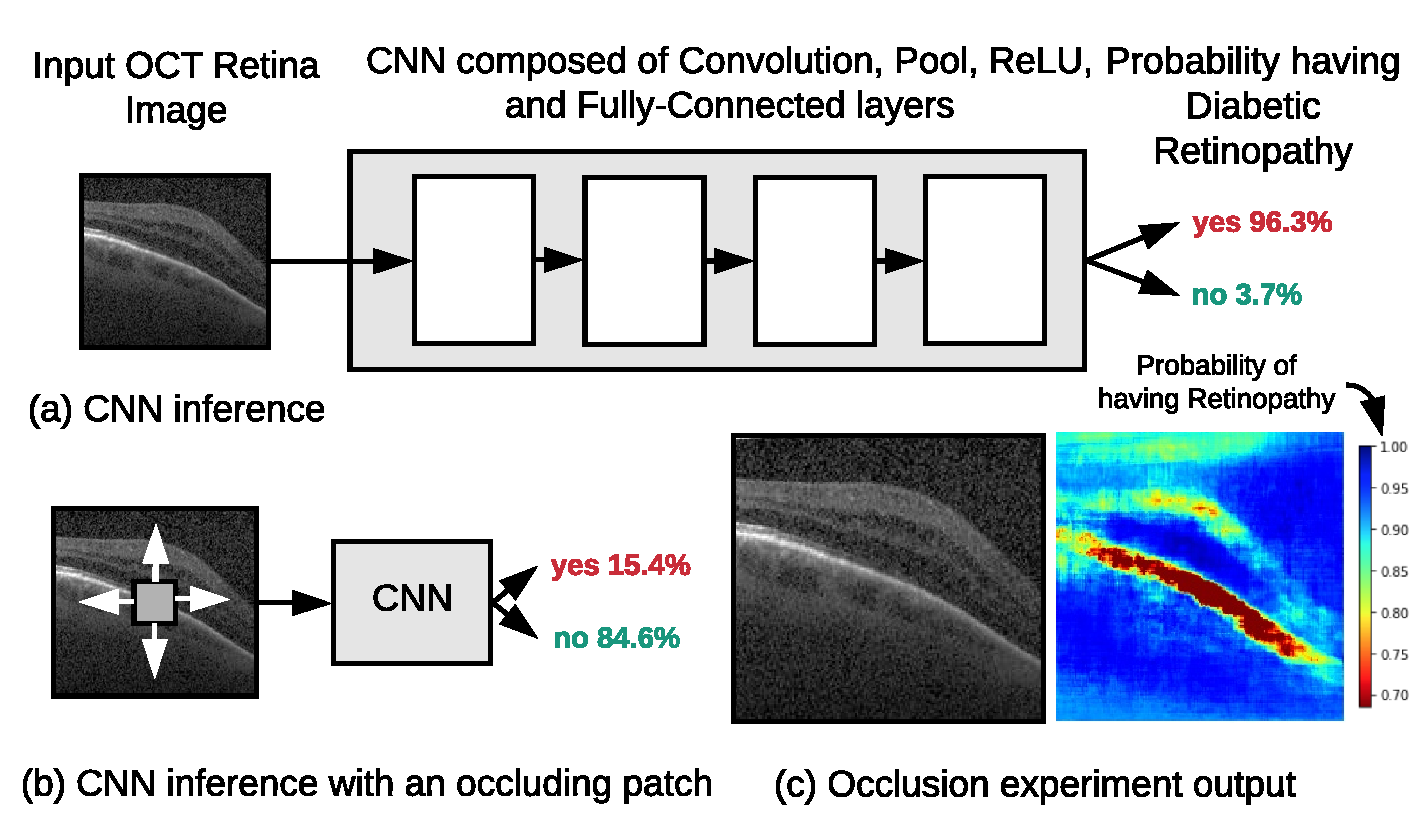
\includegraphics[width=\columnwidth]{./images/krypton_overview}
\caption{(a) Using a CNN to predict diabetic retinopathy in an OCT image/scan. (b) Occluding a part of the image changes the prediction probability. (c) By moving the occluding patch, a sensitivity heat map can be produced.}
\label{fig:krypton_overview}
\vspace{-4mm}
\end{figure}

Despite their successes, a key criticism of CNNs is that their internal workings are unintuitive to non-technical users. Thus, users often seek an ``explanation'' for why a CNN predicted a certain label. Explanations can help users trust CNNs~\cite{ribeiro2016should}, especially in high stakes applications such as radiology~\cite{jung2017deep}, and are a legal requirement for machine learning applications in some countries~\cite{gdpr}. How to explain a CNN prediction is still an active research question, but in the practical literature, an already popular mechanism for CNN explanations is a simple procedure called \textit{occlusion-based explanations}~\cite{zeiler2014visualizing}, or OBE for short.

OBE works as follows. Place a small square patch (usually gray or black) on the image to occlude those pixels. Rerun CNN inference, illustrated in Figure~\ref{fig:krypton_overview} (a), on the occluded image. The probability of the predicted label will change, as Figure~\ref{fig:krypton_overview} (b) shows. Repeat this process by moving the patch across the image to obtain a sensitivity \textit{heat map} of the probability changes, as Figure~\ref{fig:krypton_overview} (c) shows. This heat map will highlight regions of the image that were highly sensitive or ``responsible'' for the prediction (red/orange color regions). Such \textit{localization} of the regions of interest allows users to gain intuition on what ``mattered'' for the CNN prediction. For instance, the heat map can highlight the diseased areas of a tissue image, which a radiologist can then inspect more deeply for further tests. Overall, OBE is popular because it is easy for non-technical users to understand.

Alas, OBE is highly computationally expensive. Deep CNN inference is already expensive; OBE just amplifies it by issuing a large number of CNN re-inference requests (often 1000s)~\cite{ketkar2017introduction}. For example,~\cite{zintgraf2017visualizing} report over 500,000 re-inference requests for OBE on one image, which took 1hr even on a GPU! Such long wait times can hinder users' ability to consume explanations and reduce their productivity. One could use more compute hardware, if available, since OBE is embarrassingly parallel across re-inference requests. But throwing more machines at it may not always be affordable, especially for domain scientists, or feasible in all settings, e.g., in mobile clinical diagnosis. Using extra resources can also raise monetary costs, especially in the cloud.

In this paper, we use a database-inspired lens to formalize, optimize, and accelerate OBE. We start with a simple but crucial observation: \textit{the occluded images are not disjoint but share most of their pixels; so, most of CNN re-inference computations are redundant.} This observation leads us to connect OBE with two classical data management concerns: \textit{incremental view maintenance} (IVM) and \textit{multi-query optimization} (MQO). Instead of treating a CNN as a ``blackbox,'' we open it up and formalize \textit{CNN layers} as ``queries.'' Just like how a relational query coverts relations to other relations, a CNN layer converts \textit{tensors} (multidimensional arrays) to other tensors. So, we reimagine OBE as \textit{a set of tensor transformation queries} with incrementally updated inputs. With this fresh database-inspired view, we introduce several \textit{novel CNN-specific query optimization techniques} to accelerate OBE.

Our first optimization is \textit{incremental CNN inference}. We \textit{materialize} all tensors produced by the CNN's layers on the given image. For every re-inference request in OBE, instead of rerunning CNN inference from scratch, we treat it as an IVM query, with the ``views'' being the tensors. We rewrite such queries to \textit{reuse} as much of the materialized views as possible and recompute only what is needed, thus \textit{avoiding computational redundancy}. Such rewrites are non-trivial because they are closely tied to the complex geometric dataflows of CNN layers. We formalize such dataflows to create an \textit{algebraic framework} of CNN query rewrites. We also create a static analysis routine to predict how much computations can be saved before running any inference. Going further, we batch all re-inference requests in OBE to reuse the \textit{same} materialized views. This is a form of MQO, albeit interwoven with our IVM, leading to a novel \textit{batched incremental CNN inference} procedure. We also create a GPU-optimized kernel for our procedure. To the best of our knowledge, this is the first instance of IVM being fused with MQO in query optimization, at least for CNN inference.

We then introduce two novel \textit{approximate inference} optimizations that allow users to tolerate some degradation in visual quality of the heat maps produced to reduce runtimes further. These optimizations build upon our incremental inference optimization to trade off heat map quality in a user-tunable manner. Our first approximate optimization, \textit{projective field thresholding}, draws upon an idea from neuroscience and exploits the internal semantics of how CNNs work. Our second approximate optimization, \textit{adaptive drill-down}, exploits the semantics of the OBE task and the way users typically consume the heat maps produced. We also present intuitive automated parameter tuning methods to help users adopt these optimizations.

We prototype our ideas in the popular deep learning framework PyTorch to create a tool we call \system. It works on both CPU and GPU and currently supports a few popular deep CNNs (VGG16, ResNet18, and InceptionV3). We perform a comprehensive empirical evaluation of \system ~with three real-world image datasets from recent radiology and computer vision papers. \system ~yields up to $35$X speedups over the current dominant practice of running re-inference with just batching for producing high-quality approximate heat maps and up to $5$X speedups for producing exact heat maps. We then analyze the utility of each of our optimizations. Overall, this paper makes the following contributions:

\vspace{-2.5mm}
\begin{itemize}
	\item To the best of our knowledge, this is the first paper to formalize and optimize the execution of occlusion-based explanations (OBE) of CNN predictions from a data management standpoint.

	\item We cast OBE as an IVM problem to create a novel and comprehensive algebraic framework for incremental CNN inference. We also combine our IVM technique with an MQO-style technique to further reduce computational redundancy in CNN inference.

	\item We present two novel approximate inference optimizations for OBE that exploit the semantics of CNNs and properties of human perception.

	\item We prototype our ideas in a tool, \system, and perform an extensive empirical evaluation with real data and deep CNNs. \system ~speeds up OBE by even over an order of magnitude in some cases.

\end{itemize}

\vspace{-2.5mm}
\noindent \textbf{Outline.} 
Section 2 explains our problem setup, assumptions, formalization of the dataflow of CNNs. Section 3 presents our incremental inference and multi-query optimizations. Section 4 presents our approximate inference optimizations. Section 5 presents the experiments. We discuss other related work in Section 6 and conclude in Section 7.


\section{Background}

\vspace{2mm}
\noindent \textbf{Deep CNNs.} Deep CNNs are a type of neural networks specialized for image data.
They exploit spatial locality of information in image pixels to construct a hierarchy of parametric feature extractors and transformers organized as layers of various types: \textit{convolutions}, which use image
filters from graphics, except with variable filter weights, to extract features; \textit{pooling}, which subsamples features in a spatial
locality-aware way; \textit{batch-normalization}, which normalizes the output of the layer; \textit{non-linearity}, which applies a non-linear transformation (e.g., ReLU); \textit{fully connected}, which is a multi-layer perceptron; and \textit{softmax}, which emits predicted probabilities to each class label.
In most ``deep'' CNN architectures, above layers are simply stacked together with ones output is simply fed as the input to the other, while adding multiple layers element-wise or stacking multiple layers together to produce a new layer is also present in some architectures.
Popular deep CNN model architectures include AlexNet \cite{alexnet}, VGG \cite{vggnet}, Inception~\cite{inception}, ResNet~\cite{resnet}, SqueezeNet~\cite{squeezenet}, and MobileNet~\cite{mobilenets}.

% In this work, the discussion and evaluation is focused on VGG-16 (16 layer version), ResNet-18 (18 layer version) and Inception-V3 (version 3) which are three widely used CNN models in real world transfer learning applications.
% Nevertheless, our work is orthogonal to the specifics of a particular architecture and the proposed approaches can be easily extended to any architecture.

\vspace{2mm}
\noindent \textbf{Deep CNN Explainability} With image classification models, natural question is if the model is truly identifying objects in the image or just using surrounding or other objects for making false prediction.
The various approaches used to explain CNN predictions can be broadly divided into two categories, namely gradient based and perturbation based approaches. Gradient based approaches generate a sensitivity map by computing the partial derivatives of model output with respect to every input pixel via back propagation.
In perturbation based approaches the output of the model is observed by masking out regions in the input image and there by identify the sensitive regions. The most popular perturbation based approach is occlusion experiments which was first introduced by Zeiler et. al. \cite{zeiler2014visualizing}.
Even though gradient approaches require only a single forward inference and a single backpropagation to generate the sensitivity map, the output may not be very intuitive and hard to understand because the salient pixels tend to spread over a very large are of the input image.
Also the back-propagation based methods are based on the AI researchers’ intuition of what constitutes a “good” explanation. But if the focus is on explaining decision to a human observer, then the approach used to produce the explanation should have a structure that humans accept~\cite{miller2017explanation}.
As a result in most real world use cases such as in medical imaging, practitioners tend to use occlusion experiments as the preferred approach for explanations as they produce high quality fine grained sensitivity maps despite being time consuming~\cite{jung2017deep}.

Over the years there has been several modifications proposed to the original occlusion experiment approach. More recently Zintgraf. et. al. \cite{zintgraf2017visualizing} proposed a variation to the original occlusion experiment approach named \textit{Prediction Difference Analysis}. In this method instead of masking with a grey or black patch, samples from surrounding regions in the image are chosen as occlusion patches.
In our work we mainly focus on the original occlusion experiment method. But, the methods and optimizations proposed in our work are readily applicable to more advanced occlusion based explainability approaches.

%!TEX root = <main.tex>
\section{Preliminaries and Overview}\label{sec:preliminaries}
In this section, we first formally state the problem and explain our assumptions.
Then we formalize the internals of critical layers in a deep CNN for the purpose of proposing our \textit{incremental inference} approach in Section 4.
\eat{
Finally we briefly explain the Structural Similarity Index (SSIM) which is used to quantify the quality of the generated sensitivity heat maps.
}

\subsection{Problem Statement and Assumptions}\label{sec:problem}

\begin{table}[t]
  \centering
  \caption{Symbols used in the Section 3}
  \scalebox{0.8}{\begin{tabular}{p{2cm}p{7.5cm}}
    \toprule
    \textbf{Symbol} & \textbf{Meaning}\\
    \midrule \midrule
    $f$ & Fine-tuned CNN which takes in an input image and outputs a probability distribution over the class labels\\
    \midrule
    $T_{:l}$ & Tensor transformation function used in the $l^{th}$ layer of the CNN $f$\\
    \midrule
    $L$ & Class label predicted by $f$ for the original image $\mathcal{I}_{:img}$\\
    \midrule
    $\mathcal{P}$ & Occluding patch in RGB format\\
    \midrule
    $S_\mathcal{P}$ & Occluding patch striding amount\\
    \midrule
    $G$ & Set of occluding patch superimposition positions on $\mathcal{I}_{:img}$ in (x,y) format\\
    \midrule
    $M$ & Heat map produced by the occlusion experiment\\
    \midrule
    $H_M,W_M$ & Height and width of $M$\\
    \midrule
    $\bm\circ_{x,y}$ & Superimposition operator. $A~\circ_{x,y}~B$, superimposes $B$ on top of $A$ starting off at $(x,y)$ position\\
    \midrule
    $\mathcal{I}_{:l} (\mathcal{I}_{:img})$ & Input tensor of the $l^{th}$ layer (Input Image)\\
    \midrule
    $\mathcal{O}_{:l}$ & Output tensor of the $l^{th}$ layer\\
    \midrule
    $C_{\mathcal{I}:l},H_{\mathcal{I}:l},W_{\mathcal{I}:l}$ & Depth, height, and width of $l^th$ layer Input\\
    \midrule
    $C_{\mathcal{O}:l},H_{\mathcal{O}:l},W_{\mathcal{O}:l}$ & Depth, height, and width of $l^{th}$ layer Output\\
    \midrule
    $\mathcal{K}_{conv:l}$ & Convolution filter kernels for the $l^{th}$ layer\\
    \midrule
    $\mathcal{B}_{conv:l}$ & Convolution bias value vector for the $l^{th}$ layer\\
    \midrule
    $\mathcal{K}_{pool:l}$ & Pooling filter kernel for the $l^{th}$ layer\\
    \midrule
    $H_{\mathcal{K}:l},W_{\mathcal{K}:l}$ & Height and width of the filter kernel for the $l^{th}$ layer\\
    \midrule
    $S_{:l}$$\equiv$$(S_{x:l},S_{y:l})$ & Filter kernel patch striding amount for the $l^{th}$ layer ($S_{x:l}$ and $S_{y:l}$ corresponds to width and height dimensions)\\
    \midrule
    $P_{:l}$$\equiv$$(P_{x:l},P_{y:l})$ & Padding amount for the $l^{th}$ layer ($P_{x:l}$ and $P_{y:l}$ corresponds to padding along width and height dimensions)\\
    % $Q (Q_{inc})$ & Total FLOPS count with full (incremental) inference\\
    % \midrule
    % $L$ & Set of convolution layers in a CNN\\
    % \midrule
    \bottomrule
  \end{tabular}}
\label{table:preliminaries_symbols}
\end{table}

We are given a CNN $f$ which consists of a sequence or a DAG of tensor transformation functions $T_{:l}$s, an image $\mathcal{I}_{:img}$ on which the occlusion experiment needs to be run, the predicted class label $L$ for $\mathcal{I}_{:img}$, an occluding patch $\mathcal{P}$ in RGB format, and occluding patch striding amount $S_{\mathcal{P}}$.
We are also given a set of interested occluding patch positions $G$, constructed either automatically or by the human with a visual interface interactively.
The occlusion experiment workload is to generate a 2-D heat map $M$, where each value correspond to the coordinates in $G$ contains the predicted probability for $L$ by $f$ for the occluded image $\mathcal{I}^{'}_{x,y:img}$ or zero otherwise.
More precisely, we can state the workload using the following set of logical statements:

\begin{align}
\label{eqn:mheight}
W_M =&~ \lfloor(\texttt{width}(\mathcal{I}_{:img}) - \texttt{width}(\mathcal{P}) + 1)/S_\mathcal{P}\rfloor\\
\label{eqn:mwidth}
H_M =&~ \lfloor(\texttt{height}(\mathcal{I}_{:img}) - \texttt{height}(\mathcal{P}) + 1)/S_\mathcal{P}\rfloor\\
M \in&~ \mathcal{\rm I\!R}^{H_M \times W_M}\\
\forall~ x,y \in&~ G:\\
\label{eqn:patchimpose}
& \mathcal{I}^{'}_{x,y:img} \leftarrow \mathcal{I}_{:img} ~ \bm\circ_{x,y} ~ \mathcal{P} \\
\label{eqn:outputval}
& M[x,y] \leftarrow f(\mathcal{I}^{'}_{x,y:img})[L]
\end{align}


Step (\ref{eqn:mheight}), and (\ref{eqn:mwidth}) calculates the dimensions of the generated heat map $M$ which is dependent on the dimensions of $\mathcal{I}_{:img}$, $\mathcal{P}$, and $S_\mathcal{P}$.
Step (\ref{eqn:patchimpose}) superimposes $\mathcal{P}$ on $\mathcal{I}_{:img}$ with its top left corner placed on the (x,y) location of $\mathcal{I}_{:img}$.
Step (\ref{eqn:outputval}) calculates the output value at the (x,y) location by performing CNN inference for $\mathcal{I}^{'}_{x,y:img}$ using $f$ and picking the predicted probability for the label $L$.
Step (\ref{eqn:patchimpose}) and (\ref{eqn:outputval}) are run for all occluding patch position values in $G$.
In the non-interactive mode $G$ is initialized to $G = [0, H_M) \times [0, W_M)$, which corresponds to the set of all possible occlusion patch positions on  $\mathcal{I}_{:img}$.
In the interactive mode it is possible that human operator would provide multiple $G$s, one after the other, for which the system has to evaluate iteratively.

We assume that $f$ is a CNN from a roster of well-known CNNs (currently, we support VGG 16-layer version, ResNet 18-layer version, and Inception version 3).
We think this is a reasonable start, since most recent CNN-based image recognition applications use only such well-known CNNs from model zoos \cite{caffemodelzoo, tfmodelzoo}.
Nevertheless, our work is orthogonal to the specifics of a particular CNN architecture, and our proposed techniques can be easily extended to any CNN architecture.
We leave support for arbitrary CNNs to future work.

\subsection{Deep CNN Internals}
Input and output of individual layers in a deep CNN, except for Fully-Connected ones, are arranged into 3-D tensors that have a width, height, and depth.
For example an RGB input image of 224$\times$224 dimensions can be considered as an input tensor having a width and height of 224 and a depth of 3.
Every non-Fully-Connected layer will take in an input tensor and transform it into another tensor.
A Fully-Connected layer takes in a 1-D tensor or a flattened 3-D tensor as input and transforms it into another 1-D tensor.
For our purpose, these transformations can be broadly divided into three categories based on their spatial locality:

\begin{figure*}[t]
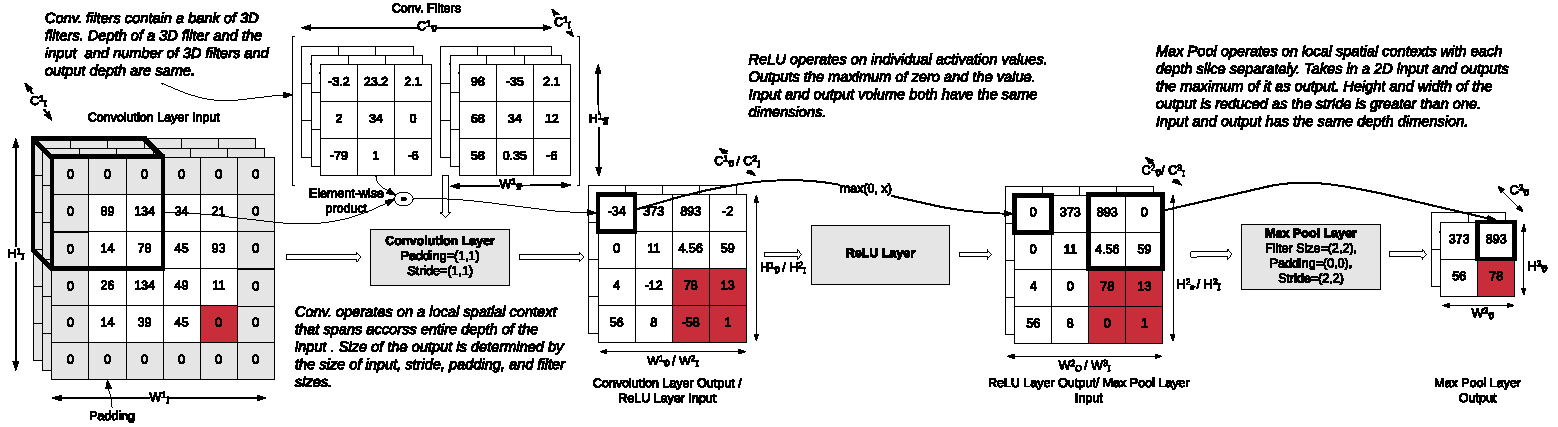
\includegraphics[width=\textwidth]{images/cnn_simplified}
\caption{Simplified representation of selected layers of a Deep CNN. The values marked in red show how a small spatial update in the first input would propagate through subsequent layers. (a) Convolution layer (for simplicity addition of bias is not shown in the Convolution transformation), (b) ReLU layer, and (c) Pool layer. Notation is explained in Table ~\ref{table:preliminaries_symbols}.}
\label{fig:cnn_simplified}
\end{figure*}

\begin{itemize}
    \item Transformations that operate at the granularity of a global context.
    \begin{itemize}
     \item E.g. Fully-Connected
    \end{itemize}
	\item Transformations that operate at the granularity of individual  spatial locations.
	\begin{itemize}
	 \item E.g. ReLU, Batch Normalization
	\end{itemize}
	\item Transformations that operate at the granularity of a local spatial context.
	\begin{itemize}
	 \item E.g. Convolution, Pooling
	\end{itemize}
\end{itemize}

\vspace{2mm}
\noindent \textbf{Transformations that operate at the granularity of a global context.} These transformations operate on a global context and does not take into account the spatial information.
Fully-Connected, which is the only global transformation layer in a CNN, takes in a 1-D tensor or a flattened 3-D tensor and performs a matrix-vector multiplication with a weight matrix and produces an output 1-D tensor.
Since it performs one bulk transformation, there is almost no substantial opportunity for exploiting redundancies with incremental computations.
The computational cost of a Full-Connected transformation is proportional to the product of the size of the input and output 1-D tensors.
Fully-Connected layers are used as the last or last few layers in a CNN and only accounts for a small fraction of the total computational cost.
Thus we ignore them henceforth.

\vspace{2mm}
\noindent \textbf{Transformations that operate at the granularity of individual  spatial locations.} These transformations essentially perform a $map(.)$ function on each individual element in the tensor (see Figure \ref{fig:cnn_simplified} (b)).
Hence, the output will have the same dimensions as input.
The computational cost incurred by these transformations is proportional to the volume of the input (or output).
However, with incremental spatially localized updates in the input, such as placing an occlusion patch, only the updated region needs to be recalculated.
Extending these transformations to become change aware is straightforward since they are element-wise operations.
The computational cost of the change aware incremental transformation is proportional to the volume of only the modified region.


\vspace{2mm}
\noindent \textbf{Transformations that operate at the granularity of a local spatial context.}
With incremental spatially localized updates in the input, transformations that operate at the granularity of a local spatial context also provide opportunities for exploiting redundancy and can be made change aware.
However, with local context transformations, such as Convolution and Pooling, this extension is non-trivial due to the overlapping nature of the spatial contexts.
% Convolution layers are the most important type of layer in the CNN architecture which also contributes to most of the computational cost.

Each Convolution layer can have $C_{\mathcal{O}:l}$ 3-D ``filter kernels'' organized into a 4-D array $\mathcal{K}_{conv:l}$, with each having a smaller spatial width $W_{\mathcal{K}:l}$ and height $H_{\mathcal{K}:l}$ compared to the width $W_{\mathcal{I}:l}$ and height $H_{\mathcal{I}:l}$ of the input tensor $\mathcal{I}_{:l}$, but has the same depth $C_{\mathcal{I}:l}$.
During inference, $c^{th}$ filter kernel is ``strided'' along the width and height dimensions of the input and a 2-D ``activation map'' $A_{:c}=(a_{y,x:c})\in \mathcal{\rm I\!R}^{H_{\mathcal{O}:l} \times~ W_{\mathcal{O}:l}}$ is produced by calculating element-wise products between the kernel and the input and adding a bias value as per Equation (\ref{eqn:elementwise_product}).
The computational cost of each of these individual element-wise products is proportional to the volume of the filter kernel.
Finally, these 2-D activation maps are stacked together along the depth dimension to produce an output tensor $\mathcal{O}_{:l} \in \mathcal{\rm I\!R}^{C_{\mathcal{O}:l} \times H_{\mathcal{O}:l} \times W_{\mathcal{O}:l}}$ as per Equation (\ref{eqn:conv_operator}).
A simplified representation of Convolution transformation is shown in Figure \ref{fig:cnn_simplified} (a).


\begin{align}
\label{eqn:elementwise_product}
\begin{split}
a_{y,x:c} =& \sum_{k=0}^{C_{\mathcal{I}:l} } \sum_{j=0}^{H_{\mathcal{K}:l}-1} \sum_{i=0}^{W_{\mathcal{K}:l}-1} \mathcal{K}_{conv:l}[c, k, j, i] \\
& \quad \times \mathcal{I}_{:l}[k,y-\floor{\frac{H_{\mathcal{K}:l} }{2}}+j,x-\floor{\frac{W_{\mathcal{K}:l} }{2}}+i] \\
& \quad + \mathcal{B}_{conv:l}[c]
\end{split}
\end{align}

\begin{align}
\label{eqn:conv_operator}
\begin{split}
\mathcal{O}_{:l} = [A_{:0}, A_{:1}, ... , A_{(C_{\mathcal{O}:l}-1)}]
\end{split}
\end{align}


% \eat{
% \begin{align}
% \begin{split}
% \text{Input Volume}:&~ \mathcal{I} \in \mathcal{\rm I\!R}^{C_{\mathcal{I}} \times H_{\mathcal{I}} \times W_{\mathcal{I}}}\\
% \text{Convolution Filters}:&~ \mathcal{K}_{conv} \in \mathcal{\rm I\!R}^{C_{\mathcal{O}} \times C_{\mathcal{I}} \times H_{\mathcal{K}} \times W_{\mathcal{K}}}\\
% \text{Convolution Bias Vector}:&~ \mathcal{B}_{conv} \in \mathcal{\rm I\!R}^{C_{\mathcal{O}}}\\
% \text{Output Volume}:&~ \mathcal{O} \in \mathcal{\rm I\!R}^{C_{\mathcal{O}} \times H_{\mathcal{O}} \times W_{\mathcal{O}}}
% \end{split}
% \end{align}

% \begin{equation}
% \label{eqn:conv_operator}
% \begin{split}
% \mathcal{O}[c,y,x] &= \sum_{k=0}^{C_{\mathcal{I}}} \sum_{j=0}^{H_\mathcal{K}-1} \sum_{i=0}^{W_\mathcal{K}-1} \mathcal{K}_{conv}[c, k, j, i] \\ & \quad \quad \quad \times \mathcal{I}[k,y-\floor{\frac{H_\mathcal{K}}{2}}+j,x-\floor{\frac{W_\mathcal{K}}{2}}+i] + \mathcal{B}[c]
% \end{split}
% \end{equation}
% }

Pooling can also be thought of as a Convolution operation with a fixed (i.e., not learned) 2-D filter kernel $\mathcal{K}_{pool:l}$.
But unlike Convolution, Pooling operates independently on each depth slice of the input tensor.
% The two main variations of pooling layers are max pooling (takes the maximum value from the local spatial context) and average (takes the average value from the local spatial context) pooling.
A Pooling layer takes a 3-D activation tensor $\mathcal{O}_{l}$ having a depth of $C_{\mathcal{I}:l}$, width of $W_{\mathcal{I}:l}$, and height of $H_{\mathcal{I}:l}$ as input and produces another 3-D activation tensor $\mathcal{O}_{:l}$ with the same depth of $C_{\mathcal{O}:l}=C_{\mathcal{I}:l}$, width of $W_{\mathcal{O}:l}$, and height of $H_{\mathcal{O}:l}$ as the output.
Pooling kernel is generally strided with more than one pixel at a time and hence $W_{\mathcal{O}:l}$ and $H_{\mathcal{O}:l}$ are generally smaller than $W_{\mathcal{I}:l}$ and $H_{\mathcal{I}:l}$.
A simplified representation of Pooling transformation is shown in Figure \ref{fig:cnn_simplified} (c).
% Similar to Convolution, Pooling operation can be formally defined as follows:

% \begin{align}
% \text{Pool Filters}:&~ \mathcal{K}_{pool} \in \mathcal{\rm I\!R}^{H_{\mathcal{K}} \times W_{\mathcal{K}}}
% \end{align}

% \begin{equation}
% \label{eqn:pool_operator}
% \begin{split}
% \mathcal{O}[c,y,x] &= \sum_{j=0}^{H_\mathcal{K}-1} \sum_{i=0}^{W_\mathcal{K}-1} \mathcal{K}_{pool}[j, i] \\ & \quad \quad \quad \times \mathcal{I}[c,y-\floor{\frac{H_\mathcal{K}}{2}}+j,x-\floor{\frac{W_\mathcal{K}}{2}}+i]
% \end{split}
% \end{equation}

It can be seen that Convolution and Pooling transformations can be cast into a form of applying a filter along the spatial dimensions of the 3-D input tensor.
However, how each transformation operates along the depth dimension is different.
For our purpose, since we are only interested in finding the spatial propagation of the patches in the input through the consecutive layers, both of these transformations can be treated similarly.

\vspace{2mm}
\noindent \textbf{Relationship between Input and Output Dimensions.}
The output tensor's dimensions $W_{\mathcal{O}:l}$ and $H_{\mathcal{O}:l}$ are determined by the dimensions of the input tensor $W_{\mathcal{I}:l}$ and $H_{\mathcal{I}:l}$, dimensions of the filter kernel $W_{\mathcal{K}:l}$ and $H_{\mathcal{K}:l}$ and two other parameters: \textbf{stride} $S_{:l}$ and \textbf{padding} $P_{:l}$.
Stride is the number of pixel values used to move the filter kernel at a time when producing a 2-D activation map.
It is possible to have two different values, with one for the width dimension $S_{x:l}$ and one for the height dimension $S_{y:l}$.
Generally $S_{x:l} \leq W_{\mathcal{K}:l}$ and $S_{y:l} \leq H_{\mathcal{K}:l}$.
In Figure \ref{fig:cnn_simplified}, Convolution transformation uses a stride value of 1 and Pool transformation uses a stride value of 2 for both dimensions.
Sometimes, in order to control the dimensions of the output tensor to be same as the input tensor, one needs to pad the input tensor with zeros around the spatial border.
Padding $P_{:l}$ captures the number of zeros that needs to be added.
Similar to the stride $S_{:l}$, it is possible to have two separate values for padding, with one for the width dimension $P_{x:l}$ and one for the height dimension $P_{y:l}$.
In Figure \ref{fig:cnn_simplified}, Convolution transformation pads the input with one line of zeros on both dimensions.
With these parameters defined, the width (similarly height) of the output tensor can be defined as follows:

\begin{align}
\begin{split}
W_{\mathcal{O}:l} = (W_{\mathcal{I}:l} - W_{\mathcal{K}:l} + 1 + 2\times P_{x:l})/S_{x:l} \\
% ^lH_{\mathcal{O}} = (^lH_{\mathcal{I}} - ^lH_\mathcal{K} + 1 + 2\times ^lP_y)/^lS_y
\end{split}
\end{align}

\vspace{2mm}
\noindent \textbf{Computational Cost of Deep CNNs.}
Deep CNNs are highly compute-intensive.
Of all the types of layers, Convolution layers almost always contribute to $90\%$ (or more) of the computation.
Hence, we can roughly estimate the computational cost of a Deep CNN by counting the number of fused multiply-add (FMA) floating point operations (FLOPs) required by Convolution layers for a single forward pass for inference.
% and ignore the computational cost of other layers (e.g. Pooling, Fully-Connected).

For example, applying a Convolution filter having the dimensions of ($C_{\mathcal{I}:l}$, $H_{\mathcal{K}:l}$, $W_{\mathcal{K}:l}$) to compute a single value in the output tensor will require $C_{\mathcal{I}:l} \times H_{\mathcal{K}:l} \times W_{\mathcal{K}:l}$ FLOPs, each corresponding to a single element-wise multiplication.
Thus, the total amount of computations $Q_{:l}$ required by that layer in order to produce an output tensor $\mathcal{O}_{:l}$ with dimensions $C_{\mathcal{O}:l} \times H_{\mathcal{O}:l} \times lW_{\mathcal{O}:l}$, and the total amount of computations $Q$ required to process the entire set of convolution layers $L$ in the CNN can be calculated as per Equation (\ref{eqn:full_local}) and (\ref{eqn:full_all}).

\begin{align}
\label{eqn:full_local}
Q_{:l} =&~ (C_{\mathcal{I}:l} \times H_{\mathcal{K}:l} \times W_{\mathcal{K}:l}) \times (C_{\mathcal{O}:l} \times H_{\mathcal{O}:l} \times W_{\mathcal{O}:l})\\
\label{eqn:full_all}
Q =&~ \sum_{l \in L}Q_{:l}
\end{align}


\eat{
\subsection{Estimating the Quality of Generated Approximate Heat Maps}

When applying approximate inference optimizations \system~ sacrifices the the accuracy/quality of the generated heat map in favor of faster execution.
To measure this drop of accuracy we use Structural Similarity (SSIM) Index~\cite{wang2004image} which is one of the widely used approaches to measure the \textit{human perceived difference} between two similar images.
When applying SSIM index we treat the original heat map as the reference image with no distortions and the perceived image similarity of the \system~generated heat map is calculated with reference to it.
The generated SSIM index is a value between $-1$ and $1$, where $1$ corresponds to perfect similarity.
% It is important to note that, even though SSIM index value of 1 corresponds to perfect similarity, other values doesn't necessarily imply same level of perceived quality across different image pairs.
% However, if the original images are closely similar, such as in chest X-ray images, it can be assumed that this condition will hold.
Typically SSIM index values in the range of $0.90-0.95$ are used in practical applications such as image compression and video encoding as at the human perception level they produce indistinguishable distortions.
For more details on SSIM Index method, we refer the reader to the original SSIM Index paper~\cite{wang2004image}.
}



%!TEX root = <main.tex>
\section{Incremental Inference Optimizations}\label{sec:exact}
We start with a theoretical characterization of how much speedups we can expect from incremental inference for OBE. We then dive into our novel algebraic framework that enables incremental CNN inference and combine it with our multi-query optimization for OBE.

%inspired by incremental view maintenance in relational databases~\cite{ivm}. We start with a theoretical characterization of how much speedup is possible to set the expectation. We then dive into our novel algebraic framework to enable and optimize incremental inference for OBE. To the best of our knowledge, ours is the first work to combine incremental view maintenance with multi-query optimization for repeated CNN inference.

\vspace{-2mm}
\subsection{Expected Speedups}

\begin{figure}[t]
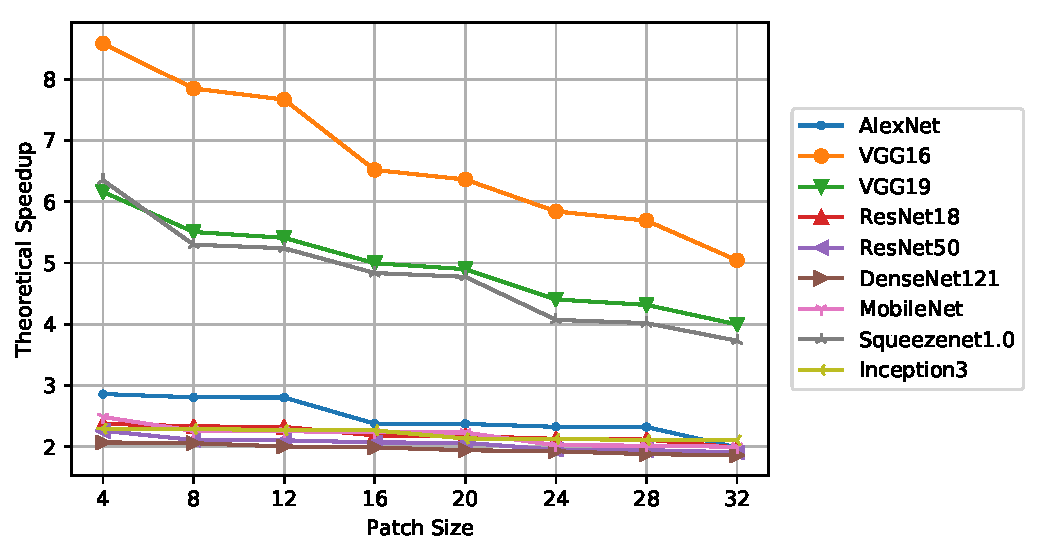
\includegraphics[width=\columnwidth]{images/redundancy_ratio}
\caption{Theoretical speedups for popular deep CNN architectures with incremental inference.}
\label{fig:redundancy_ratio}
\vspace{-8mm}
\end{figure}

The basic reason why IVM offers speedups is that when a part of the input relation is updated, IVM only computes the part of output that gets changed. We bring the IVM notion to CNNs; a CNN layer is our ``query'' and the materialized feature tensor is our ``relation.'' OBE updates only a part of the image; so, only some parts of the tensors need to be recomputed. We create an algebraic framework to determine which parts these are for a CNN layer (Section 3.2) and how to propagate updates across layers (Section 3.3). Given a CNN $f$ and the occlusion patch, our framework determines using ``static analysis'' over $f$ how many FLOPs can be saved. This gives us an upper bound on the possible speedup--we call this the ``theoretical speedup.''
%
More precisely, let the output tensor dimensions of layer $l$ be $(C_{\mathcal{O}:l} , H_{\mathcal{O}:l} , W_{\mathcal{O}:l})$. An incremental update recomputes a smaller local spatial context with width $W_{\mathcal{P}:l} \le W_{\mathcal{O}:l}$ and height $H_{\mathcal{P}:l} \le H_{\mathcal{O}:l}$. Thus, the computational cost of incremental inference for layer $l$, $Q_{inc:l}$, and the total computational cost for incremental inference for $f$, $Q_{inc}$, are given by Equations~(\ref{eqn:inc_local}) and ~(\ref{eqn:inc_all}).

\vspace{-2mm}
\begin{align}
\label{eqn:inc_local}
Q_{inc:l} =&~ (C_{\mathcal{I}:l} \cdot H_{\mathcal{K}:l} \cdot W_{\mathcal{K}:l})  (C_{\mathcal{O}:l} \cdot H_{\mathcal{P}:l} \cdot W_{\mathcal{P}:l})\\
\label{eqn:inc_all}
Q_{inc} =&~ \sum_{l~\mathit{in}~f} Q_{inc:l}
\end{align}

The above costs can be much smaller than $Q_{:l}$ and $Q$ in Equations~(\ref{eqn:full_local}) and~(\ref{eqn:full_all}) earlier.
The \textit{theoretical speedup} is defined as the ratio $\frac{Q}{Q_{inc}}$. It tells us how beneficial incremental inference can be in the best case \textit{without} performing the inference itself. It depends on several factors: the occlusion patch size, its location, the parameters of layers (kernel dimensions, stride, etc.), and so on. Calculating it is non-trivial and requires careful analysis, which we perform. The location of patch affects this ratio because a patch placed in the corner leads to fewer updates overall than one placed in the center of the image. Thus, the ``worst-case'' theoretical speedup is determined by placing the patch at the center.

We performed a sanity check experiment to ascertain the theoretical speedups for a few popular deep CNNs. For varying occlusion patch sizes (with the same stride of 1), we plot the theoretical speedups of different deep CNNs in Figure~\ref{fig:redundancy_ratio} shows the results. VGG-16 has the highest theoretical speedups, while DenseNet-121 has the lowest. Most CNNs fall in the 2X--3X range. The differences arise due to the specifics of the CNNs' architectures: VGG-16 has small Convolution filter kernels and strides, which means full inference incurs a high computational cost ($Q = 15$ GFLOPs). In turn, incremental inference is most beneficial for VGG-16. Note that we assumed an image size of $224 \times 224$ for this plot; if the image is larger, the theoretical speedups will be higher.

While one might be tempted to think that speedups of 2X-3X may not be ``that significant'' in practice, we find that they indeed are significant for at least two reasons. First, \textit{users often wait in the loop} for OBE workloads for performing interactive diagnoses and analyses. Thus, even such speedups can improve their productivity, e.g., reducing the time taken on a CPU from about 6min to just 2min, or on a GPU from 1min to just 20s. Second, and equally importantly, incremental inference is the \textit{foundation for our approximate inference} optimizations (Section 4), which amplify the speedups we achieve for OBE. For instance, the speedup for Inception3 goes up from only 2X for incremental inference to up to 8X with all of our optimizations enabled. Thus, incremental inference is critical to optimizing OBE.

\subsection{Single Layer Incremental Inference}\label{sec:inc_computation}

\begin{figure}[t]
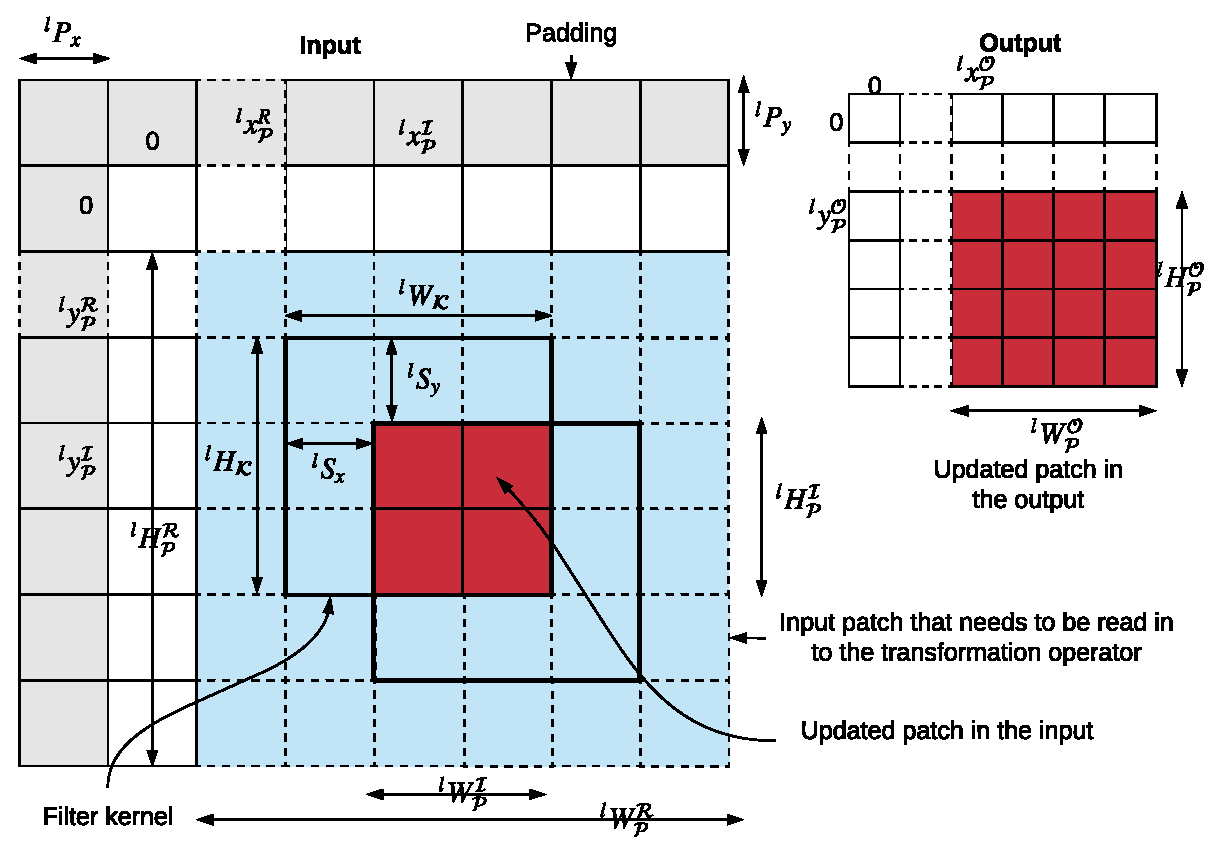
\includegraphics[width=\columnwidth]{images/dimensions}
\vspace{-8mm}
\caption{Simplified illustration of input and output update patches for Convolution/Pooling layers.}
\label{fig:dimensions}
\vspace{-8mm}
\end{figure}

We now present our algebraic framework for incremental updates to the materialized output tensor of a CNN layer. As per the discussion in Section 2.2, we focus only on the non-trivial layers that operate at the granularity of a local spatial context (Convolution and Pooling). We call our modified version of such layers ``incremental inference operations.''

\vspace{2mm}
\noindent \textbf{Determining Patch Update Locations.} We first explain how to calculate the coordinates and dimensions of the \textit{output update patch} of layer $l$ given the \textit{input update patch} and layer-specific parameters. Figure~\ref{fig:dimensions} presents a simplified illustration of these calculations. Our coordinate system's origin is at the top left corner. The input update patch is shown in red/dark color and starts at $(x^\mathcal{I}_{\mathcal{P}:l}, y^\mathcal{I}_{\mathcal{P}:l})$, with height $H^\mathcal{I}_{\mathcal{P}:l}$ and width $W^\mathcal{I}_{\mathcal{P}:l}$. The output update patch starts at $(x^\mathcal{O}_{\mathcal{P}:l}, y^\mathcal{O}_{\mathcal{P}:l})$ and has a height $H^\mathcal{O}_{\mathcal{P}:l}$ and width $W^\mathcal{O}_{\mathcal{P}:l}$. Due to overlaps among filter kernel positions during inference, computing the output update patch requires us to read a slightly larger spatial context than the input update patch--we call this the ``read-in context,'' and it is illustrated by the blue/shaded region in Figure~\ref{fig:dimensions}. The read-in context starts at $(x^\mathcal{R}_{\mathcal{P}:l}, y^\mathcal{R}_{\mathcal{P}:l})$, with its dimensions denoted by $W^\mathcal{R}_{\mathcal{P}:l}$ and $H^\mathcal{R}_{\mathcal{P}:l}$. Table~\ref{table:optimizer_symbols} summarizes all this additional notation for this section. The relationship between these quantities along the width dimension (similarly along the height dimension) can be expressed as follows:

\vspace{-4mm}
\begin{align}
\label{eqn:xcoordinate}
x^\mathcal{O}_{\mathcal{P}:l} =&~ max\big(\lceil (P_{x:l} + x^\mathcal{I}_{\mathcal{P}:l} - W_{\mathcal{K}:l} + 1)/S_{x:l} \rceil, 0\big)\\
\label{eqn:patchwidth}
W^\mathcal{O}_{\mathcal{P}:l} =&~ min\big(\lceil (W^\mathcal{I}_{\mathcal{P}:l} + W_{\mathcal{K}:l} - 1)/ S_{x:l} \rceil, W_{\mathcal{O}:l}\big)\\
\label{eqn:xreadcoordinate}
x^\mathcal{R}_{\mathcal{P}:l} =&~ x^\mathcal{O}_{\mathcal{P}:l} \times S_{x:l} - P_{x:l}\\
\label{eqn:readpatchwidth}
W^\mathcal{R}_{\mathcal{P}:l} =&~ W_{\mathcal{K}:l} + (W^\mathcal{O}_{\mathcal{P}:l}-1) \times S_{x:l}
\end{align}

% \begin{align}
% \label{eqn:xcoordinate}
% x^\mathcal{O}_\mathcal{P} =&~ max\big(\lceil (P_x + x^\mathcal{I}_\mathcal{P} - W_\mathcal{K} + 1)/S_x \rceil, 0\big)\\
% \label{eqn:ycoordinate}
% y^\mathcal{O}_\mathcal{P} =&~ max\big(\lceil (P_y + y^\mathcal{I}_\mathcal{P} - H_\mathcal{K} + 1)/S_y \rceil, 0\big)
% \end{align}

% \begin{align}
% \label{eqn:patchwidth}
% W^\mathcal{O}_\mathcal{P} =&~ min\big(\lceil (W^\mathcal{I}_\mathcal{P} + W_\mathcal{K} - 1)/S_x \rceil, W_{\mathcal{O}}\big)\\
% \label{eqn:patchheight}
% H^\mathcal{O}_\mathcal{P} =&~ min\big(\lceil (H^\mathcal{I}_\mathcal{P} + H_\mathcal{K} - 1)/S_y \rceil, H_{\mathcal{O}}\big)
% \end{align}

% \begin{align}
% \label{eqn:xreadcoordinate}
% x^\mathcal{R}_\mathcal{P} =&~ x^\mathcal{O}_\mathcal{P} \times S_x - P_x\\
% \label{eqn:yreadcoordinate}
% y^\mathcal{R}_\mathcal{P} =&~ y^\mathcal{O}_\mathcal{P} \times S_y - P_y
% \end{align}

% \begin{align}
% \label{eqn:readpatchwidth}
% W^\mathcal{R}_\mathcal{P} =&~ W_\mathcal{K} + (W^\mathcal{O}_\mathcal{P}-1) \times S_x\\
% \label{eqn:readpatchheight}
% H^\mathcal{R}_\mathcal{P} =&~ H_\mathcal{K} + (H^\mathcal{O}_\mathcal{P}-1) \times S_y
% \end{align}


Equation~(\ref{eqn:xcoordinate}) calculates the coordinates of the output update patch. Padding effectively shifts the coordinate system and thus, $P_{x:l}$ is added to correct it. Due to overlaps among the filter kernels, the affected region of the input update patch will be increased by $W_{\mathcal{K}:l}-1$, which needs to be subtracted from the input coordinate $x^\mathcal{I}_{\mathcal{P}:l}$. A filter of size $W_{\mathcal{K}:l}$ that is placed starting at $x^\mathcal{I}_{\mathcal{P}:l} - W_{\mathcal{K}:l} + 1$ will see an update starting from $x^\mathcal{I}_{\mathcal{P}:l}$. Equation~(\ref{eqn:patchwidth}) calculates the width of the output update patch. Given these, a start coordinate and width of the read-in context are given by Equations~(\ref{eqn:xreadcoordinate}) and~(\ref{eqn:readpatchwidth}); similar equations hold for the height dimension (skipped for brevity).


\begin{table}[t]
  \centering
  \scalebox{0.8}{\begin{tabular}{p{2cm}p{7.5cm}}
    \toprule
    \textbf{Symbol} & \textbf{Meaning}\\
    \midrule \midrule
    $x^\mathcal{I}_{\mathcal{P}:l}, y^\mathcal{I}_{\mathcal{P}:l}$ & Start coordinates of input update patch for layer $l$\\
    \midrule
    $x^\mathcal{R}_{\mathcal{P}:l}, y^\mathcal{R}_{\mathcal{P}:l}$ & Start coordinates of read-in context for layer $l$\\
    \midrule
    $x^\mathcal{O}_{\mathcal{P}:l}, y^\mathcal{O}_{\mathcal{P}:l}$ & Start coordinates of output update patch for layer $l$\\
    \midrule
    $H^\mathcal{I}_{\mathcal{P}:l}, W^\mathcal{I}_{\mathcal{P}:l}$ & Height and width of input update patch for layer $l$\\
   	\midrule
   	$H^\mathcal{R}_{\mathcal{P}:l}, W^\mathcal{R}_{\mathcal{P}:l}$ & Height and width of read-in context for layer $l$\\
   	\midrule
   	$H^\mathcal{O}_{\mathcal{P}:l}, W^\mathcal{O}_{\mathcal{P}:l}$ & Height and width of output update patch for layer $l$\\
    \midrule
    $\tau$ & Projective field threshold\\
    \midrule
    $r_{drill-down}$ & Drill-down fraction for adaptive drill-down\\
    \bottomrule
  \end{tabular}}
\caption{Additional notation for Sections~\ref{sec:exact} and~\ref{sec:approx}.}
\label{table:optimizer_symbols}
\vspace{-4mm}
\end{table}

\vspace{2mm}
\noindent \textbf{Incremental Inference Operation.}
For layer $l$, given the transformation function $T_{:l}$, the pre-materialized input tensor $\mathcal{I}_{:l}$, input update patch $\mathcal{P}^\mathcal{O}_{:l}$, and the above calculated coordinates and dimensions of the input, output, and read-in context, the output update patch $\mathcal{P}^\mathcal{O}_{:l}$ is computed as follows:

\vspace{-2mm}
\begin{align}
\label{eqn:readin}
\mathcal{U} =&~ \mathcal{I}_{:l}[:,x^\mathcal{R}_{\mathcal{P}:l}:x^\mathcal{R}_{\mathcal{P}:l}+W^\mathcal{R}_{\mathcal{P}:l}, y^\mathcal{R}_{\mathcal{P}:l}: y^\mathcal{R}_{\mathcal{P}:l}+ H^\mathcal{R}_{\mathcal{P}:l}]\\
\label{eqn:superposition}
\mathcal{U} =&~ \mathcal{U} \bm\circ_{(x^\mathcal{I}_{\mathcal{P}:l}-x^\mathcal{R}_{\mathcal{P}:l}),(y^\mathcal{I}_{\mathcal{P}:l}-y^\mathcal{R}_{\mathcal{P}:l})} \mathcal{P}^{\mathcal{I}}_{:l}\\
\label{eqn:callt}
\mathcal{P}^\mathcal{O}_{:l} =&~ T_{:l}(\mathcal{U})
\end{align}

Equation~(\ref{eqn:readin}) slices the read-in context $\mathcal{U}$ from the pre-materialized input tensor $\mathcal{I}_{:l}$. Equation~(\ref{eqn:superposition}) superimposes the input update patch $\mathcal{P}^\mathcal{I}_{:l}$ on it. This is an in-place update of the array holding the read-in context. Finally, Equation~(\ref{eqn:callt}) computes the output update patch $\mathcal{P}^{\mathcal{O}}_{:l}$ by invoking $T_{:l}$ on $\mathcal{U}$. Thus, we avoid performing inference on all of $\mathcal{I}_{:l}$, thus achieving incremental inference and reducing FLOPs.


\subsection{Propagating Updates across Layers}

\vspace{2mm}
\noindent \textbf{Sequential CNNs.} Unlike relational IVM, CNNs have many layers, often in a sequence. This is analogous to having a sequence of queries that require IVM on their predecessor's updated output. This leads to a new issue: correctly and automatically configuring the update patches across all layers of a CNN. Specifically, output update patch $\mathcal{P}^{\mathcal{O}}_{:l}$ of layer $l$ becomes the input update patch of layer $l+1$. While this seems simple, it requires care at the boundary of a local context transformation and a global context transformation, e.g., going from a Convolution layer (or Pooling layer) to a Fully-Connected layer. In particular, we need to materialize the \textit{full updated output} instead of propagating just the output update patches, since the global context transformation might lose spatial locality for subsequent layers.

\vspace{2mm}
\noindent \textbf{Extension to DAG CNNs.} Some recent deep CNNs have a more general directed acyclic graph (DAG) structure for layers. They have two new kinds of layers that ``merge'' two branches in the DAG: \textit{element-wise addition} and \textit{depth-wise concatenation}. Element-wise addition requires two input tensors with all dimensions being identical. Depth-wise concatenation takes two input tensors with the same height and width dimensions. We now face a new challenge--how to calculate the output update patch when the two input tensors differ on their input update patches locations and sizes? Figure~\ref{fig:la_operators} shows a simplified illustration of this issue. The first input has its update patch starting at coordinates $(x^\mathcal{I}_{\mathcal{P}_1:l},y^\mathcal{I}_{\mathcal{P}_1:l})$ with dimensions $H^\mathcal{I}_{\mathcal{P}_1:l}$ and $W^\mathcal{I}_{\mathcal{P}_1:l}$, while the second input has its update patch starting at coordinates $(x^\mathcal{I}_{\mathcal{P}_2:l},y^\mathcal{I}_{\mathcal{P}_2:l})$ with dimensions $H^\mathcal{I}_{\mathcal{P}_2:l}$ and $W^\mathcal{I}_{\mathcal{P}_2:l}$. This issue can arise with both element-wise addition and depth-wise concatenation. 

\begin{figure}[t]
\vspace{-2mm}
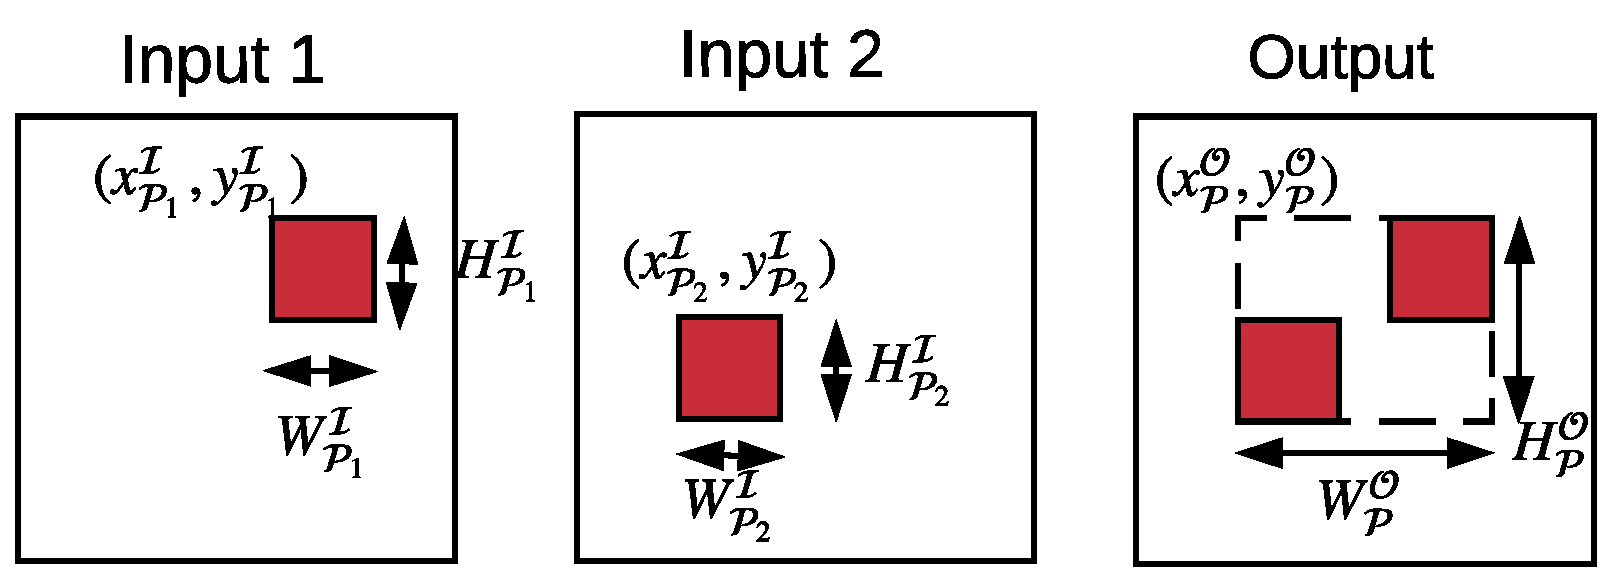
\includegraphics[width=\columnwidth]{images/la_operators}
\caption{Illustration of bounding box calculation for differing input update patch locations for element-wise addition and depth-wise concatenation layers in DAG CNNs.}
\label{fig:la_operators}
\vspace{-4mm}
\end{figure}

We propose a simple unified solution: compute the \textit{bounding box} of the input update patches. So, the coordinates and dimensions of both read-in contexts and the output update patch will be identical. Figure~\ref{fig:la_operators} illustrates this. While this will potentially recompute parts of the output that do not get modified, we think this trade-off is acceptable because the gains are likely to be marginal for the additional complexity introduced into our framework. Overall, the output update patch coordinate and width dimension are given by the following (similarly for the height dimension):

\vspace{-2mm}
\begin{align}
\begin{split}
x^\mathcal{O}_{P:l} =&~ \texttt{min}(x^\mathcal{I}_{\mathcal{P}_1:l}, x^\mathcal{I}_{\mathcal{P}_2:l})\\
% y^\mathcal{O}_\mathcal{P} = y^\mathcal{R}_\mathcal{P} =&~ \texttt{min}(y^\mathcal{I}_{\mathcal{P}_1},y^\mathcal{I}_{\mathcal{P}_2})\\
% \label{eqn:lapatchwidth}
W^\mathcal{O}_{\mathcal{P}:l} =&~ \texttt{max}(x^\mathcal{I}_{\mathcal{P}_1:l}+W^\mathcal{I}_{\mathcal{P}_1:l},x^\mathcal{I}_{\mathcal{P}_2:l}+W^\mathcal{I}_{\mathcal{P}_2:l}) -\texttt{min}(x^\mathcal{I}_{\mathcal{P}_1:l},x^\mathcal{I}_{\mathcal{P}_2:l})
% H^\mathcal{O}_\mathcal{P} = H^\mathcal{R}_\mathcal{P} =&~ \texttt{max}(y^\mathcal{I}_{\mathcal{P}_1}+H^\mathcal{I}_{\mathcal{P}_1},y^\mathcal{I}_{\mathcal{P}_2}+H^\mathcal{I}_{\mathcal{P}_2})-\texttt{min}(y^\mathcal{I}_{\mathcal{P}_1},y^\mathcal{I}_{\mathcal{P}_2})
\end{split}
\end{align}

\subsection{Multi-Query Incremental Inference}
OBE issues $|G|$ re-inference requests \textit{in one go}. Viewing each request as a ``query'' makes the connection with multi-query optimization (MQO)~\cite{sellis} clear.
The $|G|$ queries are also \textit{not disjoint}, since the occlusion patch is typically much smaller than the image, which means most the pixels are the same for each query.
Thus, we now extend our IVM framework for one re-inference with an MQO-style optimization fusing multiple re-inference requests.
An analogy with relational queries would be having many incremental update queries on the same relation in one go, with each query receiving a different incremental update. 
%To the best of our knowledge, this is the first known case of combining IVM with MQO, at least for CNN inference.

\vspace{2mm}
\noindent \textbf{Batched Incremental Inference.}
Our optimization works as follows: materialize all tensors \textit{once} and \textit{reuse} them for incremental CNN inference across all $|G|$ queries. Since most of the occluded image pixels are the identical, parts of the tensors will likely be identical too. Thus, we amortize the cost of materializing the tensors across all $|G|$ queries. One might wonder, why not just perform ``batched'' inference for the $|G|$ queries? Batched inference is standard practice today for high-throughput compute hardware like GPUs, since it amortizes CNN set up costs, data movement costs, etc. Batch sizes are picked to optimize hardware utilization. We observed that batching is an \textit{orthogonal} (albeit trivial) optimization compared to our optimization. Thus, we can combine both of these ideas to execute incremental inference in a batched manner. We call this approach ``batched incremental inference.'' Empirically, we found that batching alone yields only limited speedups (under $2$X), but combining batching and incremental inference as we do can amplify the speedups. Algorithm~\ref{alg:incinference} formally presents the batched incremental inference operation for layer $l$.

\begin{algorithm}[t]
    \caption{\textproc{BatchedIncrementalInference}}
    \label{alg:incinference}
    \begin{flushleft}
     \hspace*{1mm} \textbf{Input:} \\
     \hspace*{3mm} $T_{:l}$ : \textit{Original Transformation function}\\
     \hspace*{3mm} $\mathcal{I}_{:l}$ : \textit{Pre-materialized input from original image}\\
     \hspace*{3mm} $[\mathcal{P^I}_{1:l},...,\mathcal{P^I}_{n:l}]$ : \textit{Input patches}\\
     \hspace*{3mm} $[(x^\mathcal{I}_{\mathcal{P}_1:l},y^\mathcal{I}_{\mathcal{P}_1:l}),...,(x^\mathcal{I}_{\mathcal{P}_n:l},y^\mathcal{I}_{\mathcal{P}_n:l})]$ : \textit{Input patch coordinates}\\
     \hspace*{3mm} $W^\mathcal{I}_{\mathcal{P}:l},H^\mathcal{I}_{\mathcal{P}:l}$ : \textit{Input patch dimensions}
    \end{flushleft}

\eat{    \begin{flushleft}
     \hspace*{1mm} \textbf{Output:}\\
     \hspace*{3mm} $[\mathcal{P^O}_{1:l},...,\mathcal{P^O}_{n:l}]$ : \textit{Output patches}\\
     \hspace*{3mm} $[(x^\mathcal{O}_{\mathcal{P}_1:l},y^\mathcal{O}_{\mathcal{P}_1:l}),...,(x^\mathcal{O}_{\mathcal{P}_n:l},y^\mathcal{O}_{\mathcal{P}_n:l})]$ : \textit{Output patch coordinates}\\
     \hspace*{3mm} $W^\mathcal{O}_{\mathcal{P}:l},H^\mathcal{O}_{\mathcal{P}:l}$ : \textit{Output patch dimensions}
    \end{flushleft}}

    \begin{algorithmic}[1]
    \Procedure{BatchedIncrementalInference}{}
    \State \textit{Calculate} $[(x^\mathcal{O}_{\mathcal{P}_1:l},y^\mathcal{O}_{\mathcal{P}_1:l}),...,(x^\mathcal{O}_{\mathcal{P}_n:l},y^\mathcal{O}_{\mathcal{P}_n:l})]$ 
    \State \textit{Calculate} ($W^\mathcal{O}_{\mathcal{P}:1},H^\mathcal{O}_{\mathcal{P}:l}$)
    \State \textit{Calculate} $[(x^\mathcal{R}_{\mathcal{P}_1:l},y^\mathcal{R}_{\mathcal{P}_1:l}),...,(x^\mathcal{R}_{\mathcal{P}_n:l},y^\mathcal{R}_{\mathcal{P}_n}:l)]$
    \State \textit{Calculate} ($W^\mathcal{R}_{\mathcal{P}:l},H^\mathcal{R}_{\mathcal{P}:l}$)
    \State \textit{Initialize} $\mathcal{U} \in \mathcal{\rm I\!R}^{n \times \texttt{depth}(\mathcal{I}_{:l}) \times H^\mathcal{R}_{\mathcal{P}:l} \times W^\mathcal{R}_{\mathcal{P}:l}}$

    \For{\texttt{i in [1,...,n]}}\label{alg:line:memcpy_loop}
        \State $T_1 \gets \mathcal{I}_{:l}[:,x^\mathcal{R}_{\mathcal{P}_i:l}:x^\mathcal{R}_{\mathcal{P}_i:l}+W^\mathcal{R}_{\mathcal{P}:l},y^\mathcal{R}_{\mathcal{P}_i:l}:y^\mathcal{R}_{\mathcal{P}_i:l}+H^\mathcal{R}_{\mathcal{P}:l}]$ 
        \State $T_2 \gets T_1 \bm\circ_{(x^\mathcal{I}_{\mathcal{P}_i:l}-x^\mathcal{R}_{\mathcal{P}_i:l}),(y^\mathcal{I}_{\mathcal{P}_i:l}-y^\mathcal{R}_{\mathcal{P}_i:l})} \mathcal{P}_{i:l}$
        \State $\mathcal{U}[i,:,:] \gets T_2$
    \EndFor

    \State $[\mathcal{P}^\mathcal{O}_{1:l},...,\mathcal{P}^\mathcal{O}_{n:l}] \gets T(\mathcal{U})$ \Comment{Batched version}
    \State \textbf{return} $[\mathcal{P}^\mathcal{O}_{1:l},...,\mathcal{P}^\mathcal{O}_{n:l}]$,
    \State \hspace*{5mm} $[(x^\mathcal{O}_{\mathcal{P}_1:l},y^\mathcal{O}_{\mathcal{P}_1:l}),...,(x^\mathcal{O}_{\mathcal{P}_n:l},y^\mathcal{O}_{\mathcal{P}_n:l})],$ ($W^\mathcal{O}_{\mathcal{P}:l},H^\mathcal{O}_{\mathcal{P}:l}$) 
    \EndProcedure
    \end{algorithmic}

% \eat{%Maybe in the Appendix
%     \vspace*{-2mm}
%     \hrulefill
    
%     \begin{flushleft}
%      \hspace*{4mm} \textbf{Input:}\\
%      \hspace*{8mm} $\mathcal{O}$ : \textit{Pre-materialized output from original image}\\
%      \hspace*{8mm} $[\mathcal{P}^\mathcal{O}_1,...,\mathcal{P}^\mathcal{O}_n]$ : \textit{Output patches}\\
%      \hspace*{8mm} $[(x^\mathcal{O}_{\mathcal{P}_1},y^\mathcal{O}_{\mathcal{P}_1}),...,(x^\mathcal{O}_{\mathcal{P}_n},y^\mathcal{O}_{\mathcal{P}_n})]$ : \textit{Output patch coordinates}\\
%     \end{flushleft}

%     \begin{flushleft}
%      \hspace*{4mm} \textbf{Output:}\\
%      \hspace*{8mm} $O\textrm'$ : \textit{Updated output}
%     \end{flushleft}
%   \begin{algorithmic}[1]
%     \Procedure{IncrementalToFullProjection}{}
%     \State \textit{Initialize} $\mathcal{O}\textrm' \in \mathcal{\rm I\!R}^{n \times \texttt{depth}(\mathcal{O}) \times \texttt{height}(\mathcal{O}) \times \texttt{width}(\mathcal{O})}$
%     \For{\texttt{i in [1,...,n]}}
%       \State $T \gets \texttt{copy}(O)$
%       \State $\mathcal{O}\textrm'[i,:,:] \gets T \bm\circ_{x^\mathcal{O}_{\mathcal{P}_i},y^\mathcal{O}_{\mathcal{P}_i}} \mathcal{P}^\mathcal{O}_i$
%     \EndFor
%     \State \textbf{return} $\mathcal{O}\textrm'$
%     \EndProcedure
%     \end{algorithmic}
% }
\end{algorithm}


\eat{
The \textproc{BatchedIncrementalInference} procedure takes in the original transformation of the layer, pre-materialized input for the layer corresponding to the original image, a batch of updated patches which are 3D volumes of activation values and their geometric properties as input.
}

\textproc{BatchedIncrementalInference} first calculates the geometric properties of the output update patches and read-in contexts. A temporary tensor $U$ is initialized to hold the input update patches with their read-in contexts. The \textbf{for} loop iteratively populates $U$ with corresponding patches. Finally, $T_{:l}$ is applied to $U$ to compute the output patches. We note that only for the first layer, all input update patches will be identical to the occlusion patch. But for the later layers, the update patches will start to deviate depending on their locations and read-in contexts.


\vspace{2mm}
\noindent \textbf{GPU Optimized Implementation.}
Empirically, we found a dichotomy between CPUs and GPUs: \textproc{BatchedIncrementalInference} yielded expected speedups on CPUs, but it performed dramatically poorly on GPUs. In fact, a naive implementation of \textproc{BatchedIncrementalInference} on GPUs was \textit{slower} than full re-inference! We now shed light on why this is the case and how we tackled this issue. The \textbf{for} loop in line~\ref{alg:line:memcpy_loop} of Algorithm~\ref{alg:incinference} is essentially preparing the input for $T_{:l}$ by copying values (slices of the materialized tensor) from one part of GPU memory to another sequentially. A detailed profiling of the GPU showed that these \textit{sequential memory copies are a bottleneck} for GPU throughput, since they throttle it from exploiting its massive parallelism effectively. To overcome this issue, we created a custom CUDA kernel to perform input preparation more efficiently by \textit{copying memory regions in parallel} for all items in the batched inference request. This is akin to a parallel \textbf{for} loop tailored for slicing the tensor. We then invoke $T_{:l}$, which is already hardware-optimized by modern deep learning tools~\cite{chetlur2014cudnn}. We defer more details on our custom CUDA kernel to the appendix due to space constraints. Also, since GPU memory might not be enough to fit all $|G|$ queries, the batch size for GPU execution might be smaller than $|G|$.
%\red{TODO: Refer to hardware works, e.g. Li Tseng, Lin, Swanson, Yannis on hardware accelerators}


\vspace{-2mm}
\subsection{Putting it All Together}

We summarize the end-to-end workflow of our incremental inference optimizations for OBE. We are given the CNN $f$, image $\mathcal{I}_{:img}$, predicted class label $L$, occlusion patch $\mathcal{P}$ and its stride $S_{\mathcal{P}}$, and the set of occlusion patch positions $G$. Pre-materialize the output tensors of all layers of $f$ with $\mathcal{I}_{:img}$ as the input. Prepare occluded images ($\mathcal{I}^{'}_{(x,y):img}$) for all positions in $G$. For batches of $\mathcal{I}^{'}_{(x,y):img}$ as the input, invoke the transformations functions of the layers of $f$ in topological order and calculate the corresponding entries of heat map $M$. 
For transformations with local spatial context, invoke \textproc{BatchedIncrementalInference}. For layer that precede a global context transformation, materialize the full updated output. For all other layers, invoke the original transformation function. $M$ is now the output heat map.


\vspace{-2mm}
\section{Approximate Inference Optimizations}\label{sec:approx}
Since incremental inference is \textit{exact}, i.e., it yields the same heat map as full inference, it does not exploit a capability of human perception: tolerance of some degradation in visual quality. Thus, we now build upon our IVM framework to create two novel heuristic approximate inference optimizations that trade off the heat map's quality in a user-tunable manner to accelerate OBE further. We first explain the techniques and then explain how to tune them.

\subsection{Projective Field Thresholding}

\begin{figure}[t]
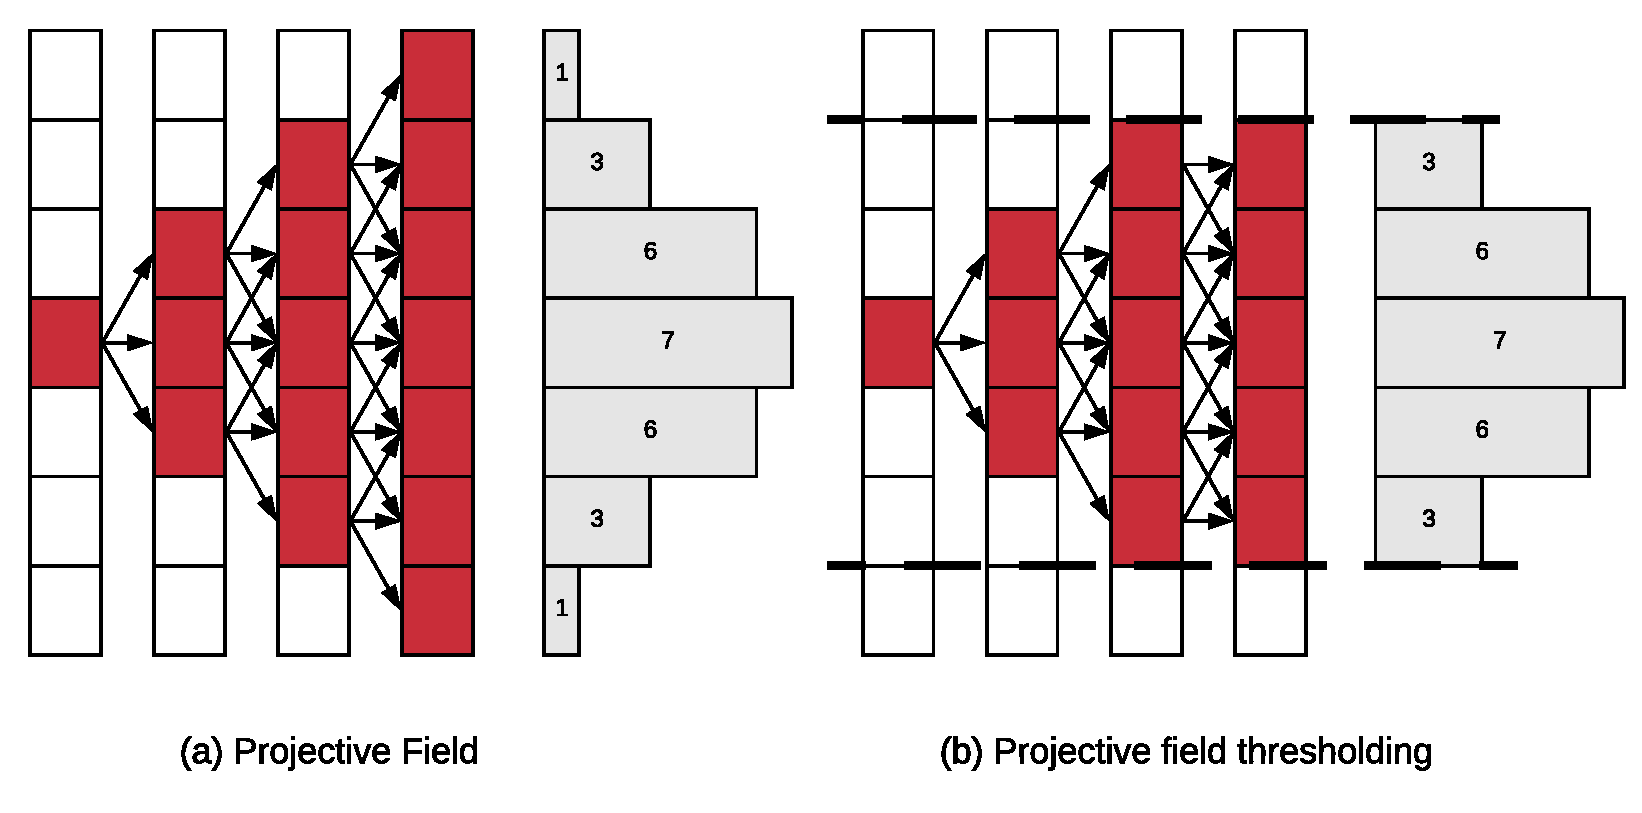
\includegraphics[width=\columnwidth]{images/pf_truncate}
\caption{(a) Projective field growth for 1-D Convolution (filter size $2$, stride $1$). (b) Projective field \textit{thresholding}; $\tau = 5/7$.}
\label{fig:pf_truncate}
\end{figure}

\begin{figure}[t]
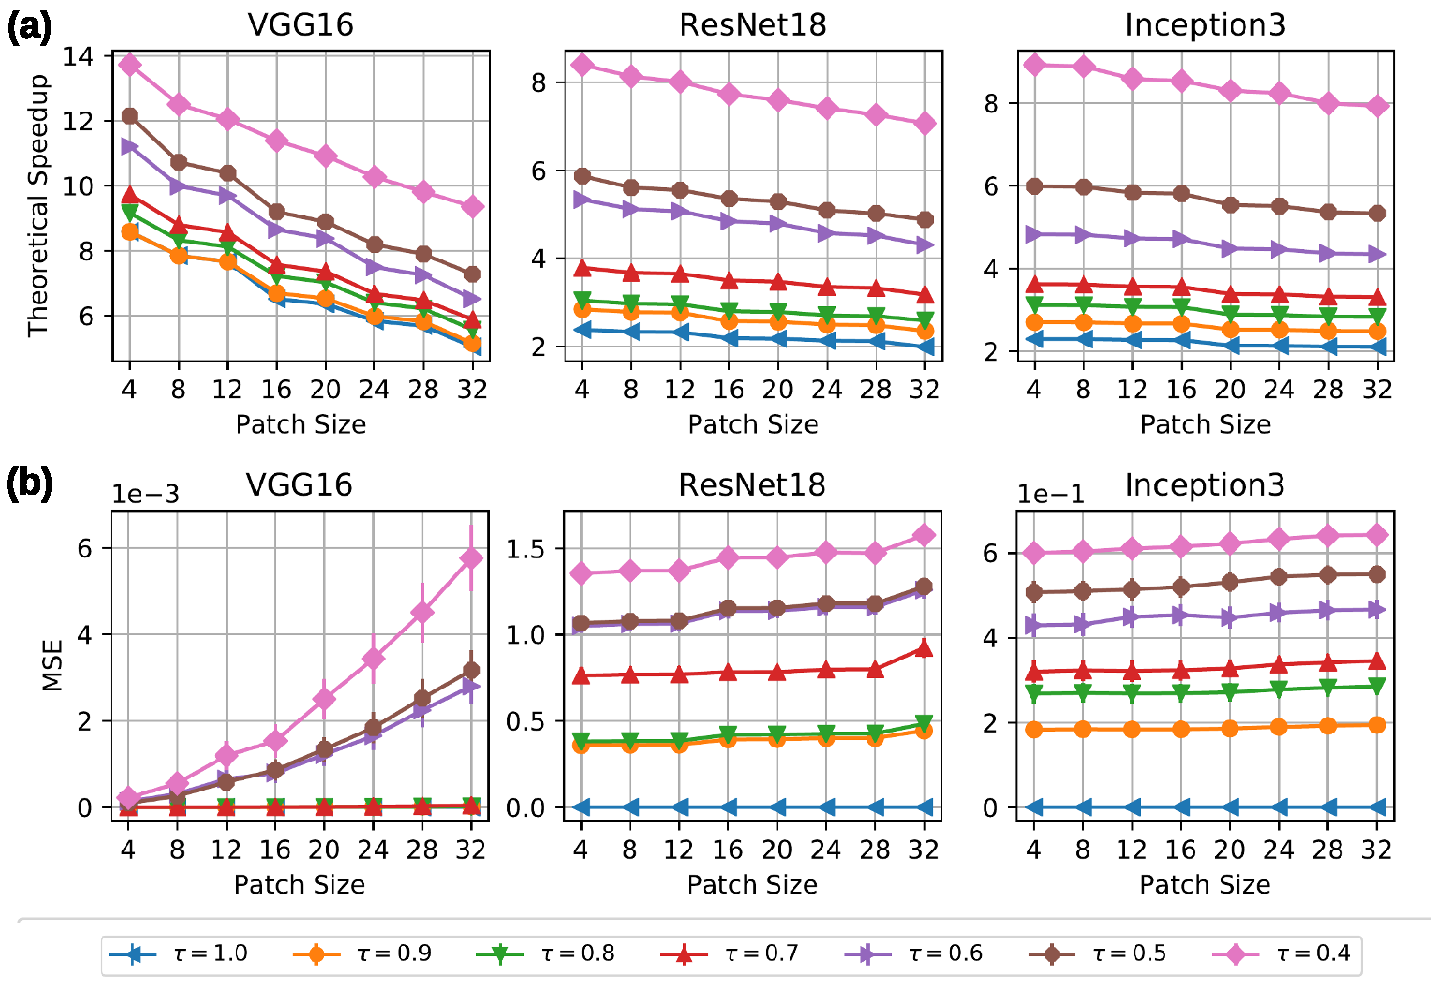
\includegraphics[width=\columnwidth]{images/proj_thresholding}
\caption{(a) Theoretical speedups with projective field thresholding. (b) Mean Square Error between exact and approximate output of final Convolution/Pooling layers.}
\label{fig:proj_thresholding}
\vspace{-4mm}
\end{figure}

The \textit{projective field} of a CNN neuron is the slice of the output tensor that is connected to it~\cite{le2017receptive, basiccnnoperations}. It is a term from neuroscience to describe the effects of a retinal cell on the output of the eye's neuronal circuitry~ \cite{de2011projective}. This notion sheds light on the \textit{growth of the size} of the update patches through the layers of a CNN. The 3 kinds of layers (Section 2.2) affect the projective field size growth differently. Transformations at the granularity of individual elements do not alter the projective field size. Global context transformations increase it to the whole output. But local spatial context transformations, which are the most crucial, increase it \textit{gradually} at a rate determined by the filter kernel's size and stride: additively in the size and multiplicatively in the stride. The growth of the projective field size implies the amount of FLOPs saved by IVM decreases as we go to the higher layers of a CNN. Eventually, the output update patch becomes as large as the output tensor. This growth is illustrated by Figure~\ref{fig:pf_truncate}(a).


Our above observation motivates the main idea of this optimization, which we call projective field thresholding: \textit{truncate} the projective field from growing beyond a given \textit{threshold fraction} $\tau$ $(0 < \tau \leq 1)$ of the output size. This means inference in subsequent layers is approximate. Figure~\ref{fig:pf_truncate}(b) illustrates the idea for a filter size 3 and stride 1. One input element is updated (shown in red/dark); the change propagates to 3 elements in the next layer and then 5, but it then gets truncated because we set $\tau = 5/7$. This approximation can alter the accuracy of the output values and this, the heat map's visual quality. Empirically, we find that modest truncation is tolerable and does not affect the heat map's visual quality too significantly. 

To provide intuition on why the above happens, consider histograms on the side of Figures~\ref{fig:pf_truncate}(a,b) that list the number of unique ``paths'' from the updated element to each element in the last layer. It resembles a Gaussian distribution, with the maximum paths concentrated on the middle element. Thus, for most of the output patch updates, truncation will only discard a few values at the ``fringes'' that contribute to an output element. Of course, we not consider the weights on these ``paths,'' which is dependent on the given trained CNN. Since the weights can be arbitrary, a tight formal analysis is unwieldy. But under some assumptions on the weights values (similar to the assumptions in~\cite{luo2016understanding} for understanding the ``receptive field'' in CNNs), we show in the appendix that this distribution does indeed converge to a Gaussian. Thus, while this idea is a heuristic, it is grounded in a common behavior of real CNNs.
\eat{
For more details we refer the reader to \cite{luo2016understanding}, where a similar theoretical result has been proved for the receptive field\footnote{Receptive field of a CNN neuron is the local region (including the depth) of the input volume which is connected to it.} of a Deep CNN.
}
Overall, since most of the contributions to the output elements are concentrated around the center, such truncation is often affordable. Note that this optimization is only feasible \textit{in conjunction with} our incremental inference framework (Section 3) to reuse the remaining parts of the tensors and save FLOPs.
We extend the formulas for the output-input coordinate calculations to account for $\tau$. For the width dimension,  the new formulas are as follows (similarly for the height dimension):

\vspace{-2mm}
\begin{align}
\label{eqn:normal_width_calc}
W^\mathcal{O}_{\mathcal{P}:l} = &~ \texttt{min}\big(\lceil (W^\mathcal{I}_{\mathcal{P}:l} + W_{\mathcal{K}:l} - 1)/S_{x:l} \rceil, W^\mathcal{O}_{\mathcal{P}:l}\big)\\
\label{eqn:check_tau}
\text{If}~ W_{\mathcal{P}:l}^\mathcal{O} & > \texttt{round}(\tau \times W^\mathcal{O}_{:l}):\\
\label{eqn:new_width_calc_with_tau}
& W^\mathcal{O}_{\mathcal{P}:l} = \texttt{round}(\tau \times W^\mathcal{O}_{:l})\\
\label{eqn:new_in_width}
& W^\mathcal{I}_{\mathcal{P}_{new}:l} = W^\mathcal{O}_{\mathcal{P}:l} \times S_{x:l} - W_{\mathcal{K}:l} + 1\\
\label{eqn:new_x_coord}
& x^{\mathcal{I}}_{\mathcal{P}:l} \mathrel{+}= (W^\mathcal{I}_{\mathcal{P}:l} - W^\mathcal{I}_{\mathcal{P}_{new}:l})/2\\
\label{eqn:new_input_width}
& W^\mathcal{I}_{\mathcal{P}:l} = W^\mathcal{I}_{\mathcal{P}_{new}:l}\\
\label{eqn:new_output_x}
x^\mathcal{O}_{\mathcal{P}:l} = & \texttt{max}\big(\lceil (P_{x:l} + x^\mathcal{I}_{\mathcal{P}:l} - W_{\mathcal{K}:l} + 1)/S_{x:l} \rceil, 0\big)
\end{align}

Equation~(\ref{eqn:normal_width_calc}) calculates the width assuming no thresholding. But if the output width exceeds the threshold, it is reduced as per Equation~(\ref{eqn:new_width_calc_with_tau}). Equation~(\ref{eqn:new_in_width}) calculates the input width that would produce an output of width $W^\mathcal{O}_{\mathcal{P}:l}$; we can think of this as making $W^{\mathcal{I}}_{\mathcal{P}:l}$ the subject of Equation~(\ref{eqn:normal_width_calc}). If the new input width is smaller than the original input width, the starting $x$ coordinate should be updated as per Equation~(\ref{eqn:new_x_coord}) s.t.~the new coordinates correspond to a ``center crop'' compared to the original. Equation~(\ref{eqn:new_input_width}) sets the input width to the newly calculated input width. Equation~(\ref{eqn:new_output_x}) calculates the $x$ coordinate of the output update patch.

\vspace{2mm}
\noindent \textbf{Theoretical Speedups.}
We modify our ``static analysis'' framework to determine the theoretical speedup of incremental inference (Section 3) to also include this optimization using the above formulas. Consider a square occlusion patch placed on the center of the input image. Figure~\ref{fig:proj_thresholding}(a) plots the new theoretical speedups for varying patch sizes for 3 popular CNNs for different $\tau$ values.
As expected, as $\tau$ goes down from $1$, the theoretical speedup goes up for all CNNs. Since lowering $\tau$ approximates the heat map values, we also plot the mean square error (MSE) of the elements of the exact and approximate output tensors produced by the final Convolution or Pooling layers on a random real-world sample image. Figure~\ref{fig:proj_thresholding}(b) shows the results. As expected, as $\tau$ drops, MSE increases. But interestingly, the trends differ across the CNNs due to their different architectural properties. MSE is especially low for VGG-16, since its projective field growth is rather slow relative to the other CNNs. We acknowledge that using MSE as a visual quality metric and tuning $\tau$ are both unintuitive for humans. We mitigate these issues in Section 4.3 by using a more intuitive quality metric and by presenting an automated tuning method for $\tau$.


\subsection{Adaptive Drill-Down}\label{sec:ada-drill-down}
This optimization is also a heuristic, but it is based on our observation about a peculiar semantics of the OBE task. It modifies the way $G$ (the set of occlusion path locations) is specified and handled, especially in the non-interactive specification mode. We explain our intuition with an example. Consider a radiologist explaining a CNN prediction for diabetic retinopathy on a tissue image. The region of interest typically occupies only a tiny fraction of the image. Thus, it is an overkill to perform regular OBE for \textit{every} patch location: most of the (incremental) inference computations are effectively ``wasted'' on uninteresting regions. In such cases, we modify the OBE workflow to produce an approximate heat map using a two-stage process, illustrated by Figure \ref{fig:adaptive_drill_down}(a).

In stage one, we produce a \textit{lower resolution} heat map by using a larger stride--we call it \textit{stage one stride} $S_1$. Using this heat map, we identify the regions of the input that see the largest drops in predicted probability of the label $L$. Given a predefined parameter \textit{drill-down fraction}, denoted $r_{drill-down}$, we select a proportional number of regions based on the probability drops. In stage two, we perform OBE only for these regions with original stride value (we also call this \textit{stage two stride}, $S_2$) for the occlusion patch to yield a portion of the heat map at the original higher resolution. Since this process ``drills down'' adaptively based on the lower resolution heat map, we call it adaptive drill-down. Note that this optimization also builds upon the incremental inference optimizations of Section 3, but it is \textit{orthogonal} to projective field thresholding and can be used in addition.

% \begin{figure}[t]
% 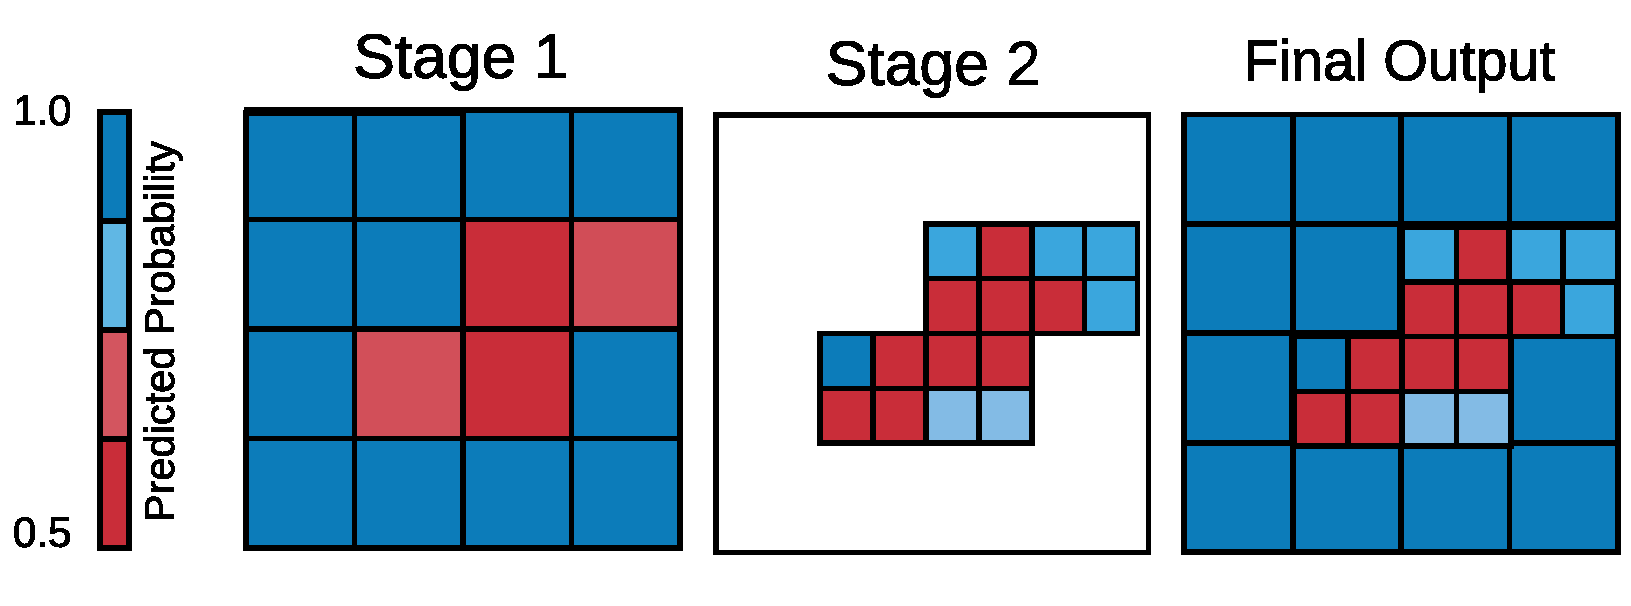
\includegraphics[width=\columnwidth]{images/adaptive-drill-down}
% \caption{Schematic representation of \textit{adaptive drill-down}}
% \label{fig:adaptive-drill-down}
% \end{figure}

\vspace{2mm}
\noindent \textbf{Theoretical Speedups.}
We now define a notion of theoretical speedup for this optimization; this is independent of the theoretical speedup of incremental inference. We first explain the effects of $r_{drill-down}$ and $S_1$. Setting these parameters is an application-specific balancing act. If $r_{drill-down}$ is low, only a small region will need re-inference at the original resolution, which will save a lot of FLOPs. But this may miss some some regions of interest and thus, compromise important explanation details. Similarly, a large $S_1$ also saves a lot of FLOPs by reducing the number of re-inference queries in stage one. But it runs the risk of misidentifying interesting regions, especially when the size of those regions are smaller than the occlusion patch size. We now define the theoretical speedup of adaptive drill-down as the ratio of the number of re-inference queries for regular OBE without this optimization to that with this optimization. We only need the counts, since the occlusion patch dimensions are unaltered, i.e., the cost of a re-inference query is the same with or without this optimization. Given a stride $S$, the number of re-inference queries is $\frac{H_{\mathcal{I}_{img}}}{S} \cdot \frac{W_{\mathcal{I}_{img}}}{S}$. Thus, the theoretical speedup is given by the following equation. Figure~\ref{fig:adaptive_drill_down}(b) illustrates how this ratio varies with $S_1$ and $r_{drill-down}$.

\vspace{-2mm}
\begin{align}
\label{eqn:adaptive-drill-down-eqn}
\texttt{speedup} = \frac{S^2_1}{S^2_2+r_{drill-down} \cdot S^2_1}
\end{align}

\begin{figure}[t]
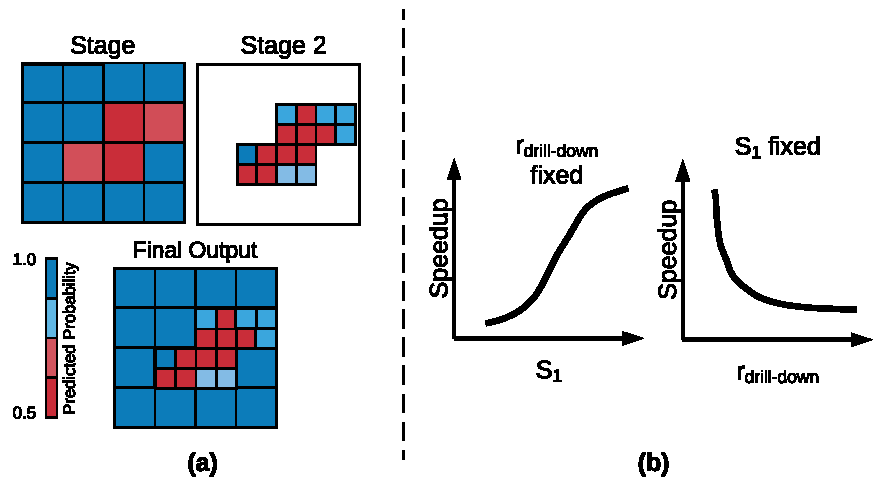
\includegraphics[width=\columnwidth]{images/adaptive_drill_down}
\caption{(a) Schematic illustration of the adaptive drill-down idea. (b) Conceptual depiction of the effects of $S_1$ and $r_{drill-down}$ on the theoretical speedup.. }
\label{fig:adaptive_drill_down}
\vspace{-4mm}
\end{figure}

\subsection{Automated Parameter Tuning}
We now present automated parameter tuning methods for easily configuring our approximate inference optimizations.

\vspace{2mm}
\noindent \textbf{Tuning projective field thresholding.}
As Section 4.1 explained, $\tau$ controls the visual quality of the heat map. There is a spectrum of visual quality degradation: imperceptible changes to major structural changes. But mapping $\tau$ to visual quality directly is likely to be unintuitive for users. Thus, to measure visual quality more intuitively, we adopt a cognitive science-inspired metric called Structural Similarity (SSIM) Index, which is widely used to quantify human-perceptible differences between two images~\cite{wang2004image}. In our case, the two ``images'' are the original and approximate heat maps. SSIM is a number in $[-1,1]$, with $1$ meaning a perfect match. SSIM values in the $[0.90,0.95]$ range are considered almost imperceptible distortions in many practical multimedia applications such as image compression and video encoding~\cite{wang2004image}.

Our tuning process for $\tau$ has an offline ``training'' phase and an online usage phase. The offline phase relies on a set of sample images (default $30$) from the same application domain. We compute SSIM for the approximate and exact heat maps for all sample images for a few $\tau$ values (default $1.0, 0.9, 0.8, \dots, 0.4$). We then learn a second-degree polynomial curve for SSIM as a function of $\tau$ with these data points. Figure~\ref{fig:system_tuning}(a) illustrates this phase and the fit SSIM-$\tau$ curves for 3 different CNNs using sample images from an OCT dataset (Section 5). In the online phase, when OBE is needed on a given image, we expect the user to provide a \textit{target SSIM} for the quality--runtime trade-off they want ($1$ yields the exact heat map). We can then use our learned curve to map this target SSIM to the lowest $\tau$. Figure~\ref{fig:system_tuning}(b) shows the CDFs of differences between the target SSIM ($0.9$) and the actual SSIM yielded when using our auto-tuned $\tau$ on both the training set and a holdout test set (also $30$ images). In $80\%$ of the cases, the actual SSIM was \textit{better} than the user-given target; never once did the actual SSIM go $0.1$ below the target SSIM. This suggests that our auto-tuning method for $\tau$ works, is robust, and applicable to different CNNs.

\vspace{2mm}
\noindent \textbf{Tuning adaptive drill-down.}
As Section~\ref{sec:ada-drill-down} explained, the speedup offered by adaptive drill-down is controlled by two parameters: stage one stride $S_1$ and drill-down fraction $r_{drill-down}$. We expect the user to provide $r_{drill-down}$ (default $0.25$), since it captures the user's intuition about how large or small the region of interest is likely to be in the images in their specific application domain and dataset. We also expect the user to provide a ``target speedup'' ratio (default $3$) for using this optimization to capture their desired quality-runtime trade-off. Higher the user's target speedup, the more we sacrifice the quality of the ``non-interesting regions'' ($1 - r_{drill-down}$ fraction of the heat map). Our automated tuning process sets $S_1$ using these two user-given settings. Unlike the tuning of $\tau$, setting $S_1$ is more direct, since this optimization relies on the number of re-inference queries, not SSIM. Let $\mathit{target}$ denote the target speedup; the original occlusion patch stride is $S_2$. Equation~\ref{eqn:s1} shows how we calculate $S_2$. Since $S_1$ cannot be larger than the image width $W_{img}$ (similarly $H_{img}$) and due to the constraint of $(1-r_{drill\-down} \cdot \texttt{speedup})$ being positive, we also have an upper bound on the possible speedups as per Equation~\ref{eqn:speedup_bound}.

\begin{align}
\label{eqn:s1}
S_1 = &~ \sqrt{\frac{\mathit{target}}{1 - r_{drill-down} \cdot \mathit{target}}} \cdot S_2
\end{align}

\vspace{-2mm}
\begin{align}
\label{eqn:speedup_bound}
\mathit{speedup} < \texttt{min}\Bigg(\frac{W^2_{img}}{S^2_2+r_{drill-down} \cdot W^2_{img}}, \frac{1}{r_{drill-down}}\Bigg)
\end{align}


\begin{figure}[t]
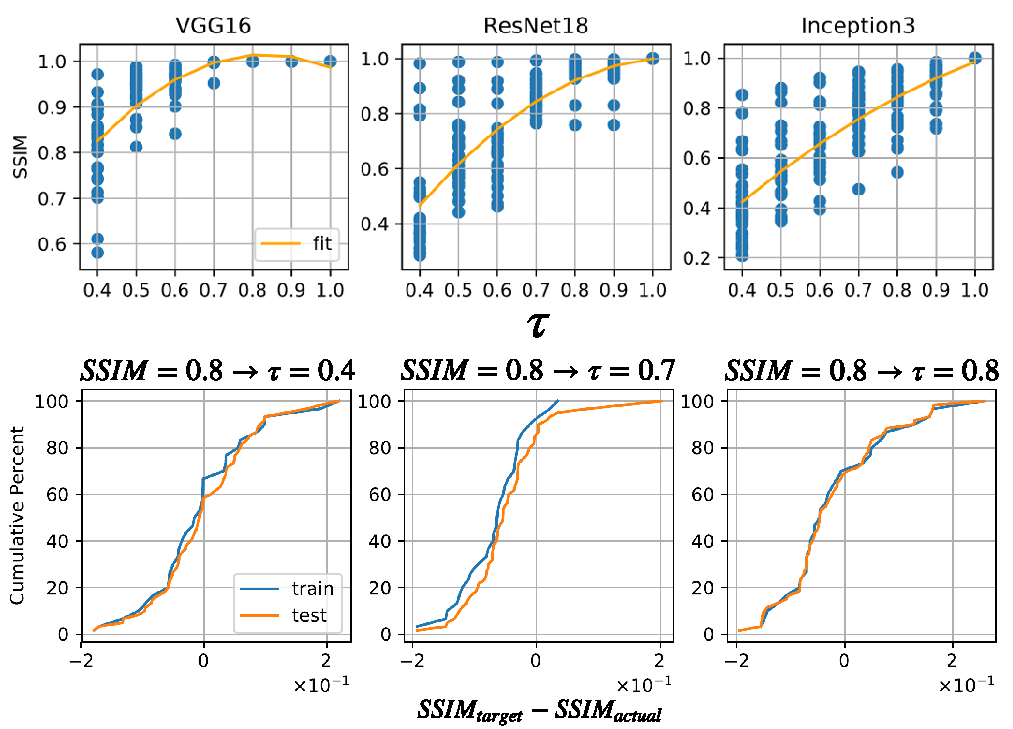
\includegraphics[width=\columnwidth]{images/system_tuning}
\caption{(a) Fitting a second-order curve for SSM against $\tau$ on a sample of the OCT dataset. 
(b) CDFs of deviation of actual SSIM from the target SSIM ($0.9$) with our auto-tuned $\tau$, which turned out to be $0.5$, $0.7$, and $0.9$ for VGG-16, ResNet-18, and Inception-V3, respectively.}
\label{fig:system_tuning}
\vspace{-4mm}
\end{figure}

% \begin{figure}[t]
% 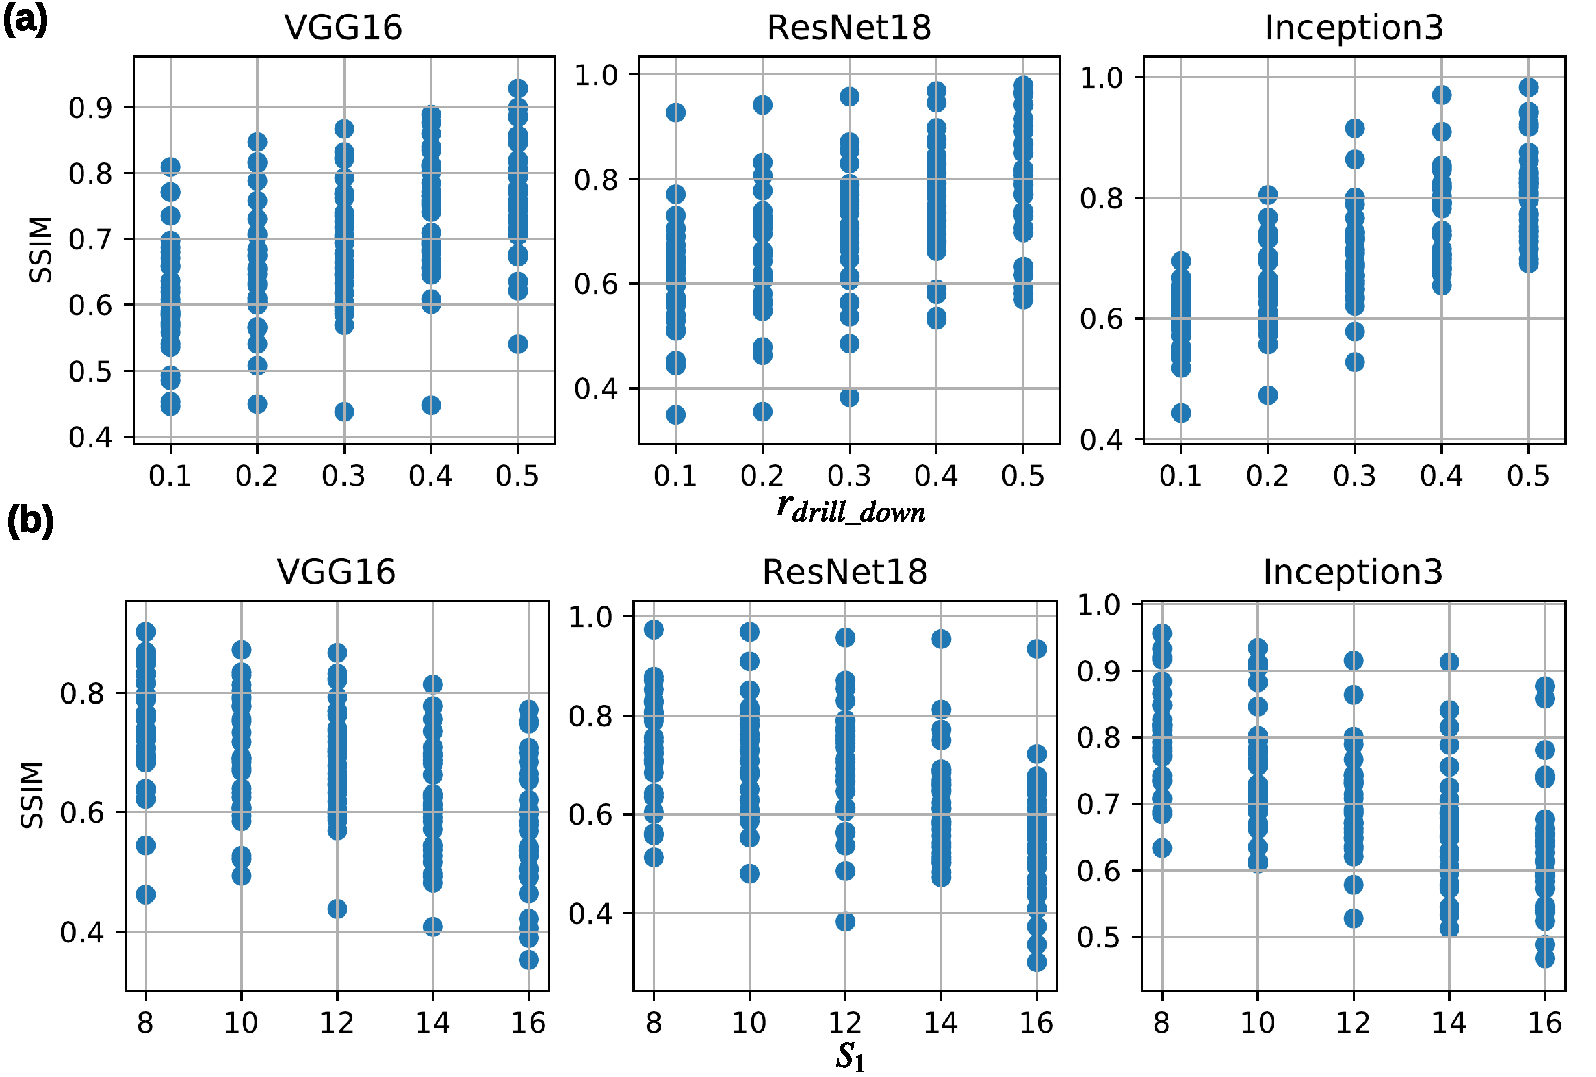
\includegraphics[width=\columnwidth]{images/adaptive_ssim}
% \caption{(a) SSIM variation for changing $r_{drill\_down}$ fixing $\tau=1$, $S_1=12$, and $S_2=4$. (b) SSIM variation for changing $S_1$ fixing $\tau=1.0$, $S_2=4$, and $r_{drill\_down}=0.3$ for a sample $(n=30)$ of OCT dataset.}
% \label{fig:adaptive_ssim}
% \end{figure}



%!TEX root = <main.tex>
\section{Experimental Evaluation}
We have integrated all of our optimization techniques from Sections 3 and 4 with the popular deep learning tool PyTorch to create a prototype tool we call \system.
We now evaluate the speedups yielded by \system~ for occlusion-based explanations for several deep CNNs on real-world image datasets.
We then drill into the contributions of each of our optimization techniques.

\vspace{2mm}
\noindent \textbf{Datasets.}
We use three diverse real-world image datasets: \textit{OCT}, \textit{Chest X-Ray}, and a sample from \textit{ImageNet}. \textit{OCT} has about 84,000 optical coherence tomography retinal images with four classes: CNV, DME, DRUSEN, and NORMAL. CNV (choroidal neovascularization), DME (diabetic macular edema), and DRUSEN are three varieties of diabetic retinopathy. NORMAL corresponds to healthy retinal images. \textit{Chest X-Ray} has about 6,000 X-ray images with three classes: VIRAL, BACTERIAL, and NORMAL. VIRAL and BACTERIAL are two varieties of pneumonia. NORMAL corresponds to healthy people. Both \textit{OCT} and \textit{Chest X-Ray} are from a recent scientific study that applied deep CNNs to radiology images to detect the respective diseases~\cite{kermany2018identifying}. \textit{ImageNet} is a benchmark dataset in computer vision~\cite{deng2009imagenet}; our sample has 1,000 images with 200 classes.

\vspace{2mm}
\noindent \textbf{Workloads.}
We use 3 popular ImageNet-trained deep CNNs: VGG16~\cite{vggnet}, ResNet18~\cite{resnet}, and Inception3~\cite{inception}, obtained from~\cite{torchvisionmodels}. They complement each other in terms of model size, architecture complexity, computational cost, and our predicted theoretical speedups for OBE with incremental inference (Figure 3 in Section 3). For \textit{OCT} and \textit{Chest X-Ray}, the 3 CNNs were fine-tuned by retraining their final Fully-Connected layers as per standard practice. The details of fine-tuning are not relevant for the rest of our discussion; so, we present further details in the Appendix. The OBE heat maps are plotted using Python Matplotlib's \texttt{imshow} method using the \texttt{jet\_r} color scheme; we set the maximum threshold to \texttt{min}$(1, 1.25 p)$ and minimum to $0.75 p$, where $p$ is predicted class probability on a given image. All images are resized to the input size required by the CNNs ($224\times224$ for VGG16 and ResNet18; $299\times299$ for Inception3); no additional pre-processing was done. The GPU-based experiments used a batch size of $128$; for CPUs, the batch size was $16$. All CPU-based experiments were executed with a thread parallelism of $8$. All of our datasets, experimental scripts, and the \system~ codebase will be made publicly available on our project webpage.

\vspace{2mm}
\noindent \textbf{Experimental Setup.}
We use a machine with 32 GB RAM, Intel i7-6700 3.40GHz CPU, and NVIDIA Titan X (Pascal) GPU with 12 GB memory. %1 TB Seagate ST1000DM010-2EP1
The machine runs Ubuntu 16.04 with PyTorch version 0.4.0, CUDA version 9.0, and cuDNN version 7.1.2.
All reported runtimes are the average of 3 runs, with 95\% confidence intervals shown.

\subsection{End-to- End Runtimes}

\begin{figure*}[t]
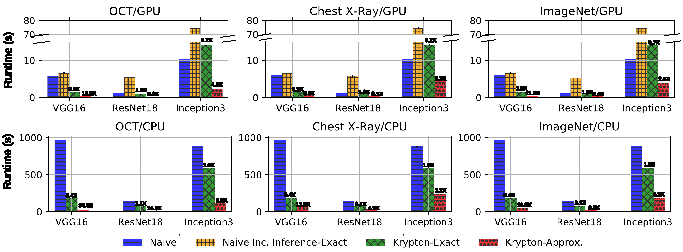
\includegraphics[width=\textwidth]{images/5_1_all_edited_b}
\vspace{-6mm}
\caption{End-to-end runtimes of \system~ and baselines on all 3 datasets, 3 CNNs, and both GPU and CPU.}
\label{fig:5_1_all_edited}
\end{figure*}

We focus on the most common OBE scenario of producing the whole heat map, i.e., $G$ is automatically created (``non-interactive'' mode). We use an occlusion patch of size 16 and stride 4. We compare two variants of \system: \system-Exact uses only incremental inference (Section 3), while \system-Approximate uses our approximate inference optimizations too (Section 4). The main baseline is \textit{Naive}, the current dominant practice of performing full inference for OBE with just naive batching of images. We have another baseline for the GPU environment: \textit{Naive Inc.~Inference-Exact}, which is a direct implementation of Algorithm~\ref{alg:incinference} in PyTorch/Python without using our GPU-optimized CUDA kernel, which \system~ uses (Section 3.4). Note that \textit{Naive Inc.~Inference-Exact} is not applicable to the CPU environment.

We set the user-given tuning parameters for adaptive drill-down based on the semantics of each dataset's prediction task (Section 4.3). For \textit{OCT}, since the region of interest is likely to be small, we set $r_{drill-down}=0.1$ and $\mathit{target} = 5$. For \textit{Chest X-Ray}, the region of interest can be large; so, we set $r_{drill-down} = 0.4$ and $\mathit{target} = 2$. For \textit{ImageNet}, which falls in between, we use the \system~ default values of $r_{drill-down}=0.25$  and $\mathit{target} = 3$. For all experiments $\tau$ is auto-tuned with a target SSIM of $0.9$ (Section 4.3). Figure~\ref{fig:5_1_all_edited} presents the results. Visual examples of images and the heat maps produced are presented in the Appendix.

Overall, we see \system~ offers significant speedups across the board on both GPU and CPU. The highest speedups are reported by \system-Approximate on \textit{OCT} with VGG16: $16$X on GPU and $34.5$X on CPU. The highest speedups of  \system-Exact are also on VGG16: $3.9$X on GPU and $5.4$X on CPU. The speedups of \system-Exact are identical across datasets for a given CNN, since it does not depend on the image semantics, unlike \system-Approximate due to its data-dependent parameters. \system-Approximate reports the highest speedups on \textit{OCT} because our auto-tuning yielded the lowest $\tau$, highest target speedup, and lowest $r_{drill-down}$ on that dataset. 

The speedups are lower with ResNet18 and Inception3 than VGG16 due to their architectural properties (kernel filter dimensions, stride, etc.) that make the projective field grow faster. Moreover, Inception3 has a complex DAG architecture with more branches and depth-wise concatenation, which limits GPU throughput for incremental inference. In fact, \system-Exact on GPU shows a minor slow-down ($0.7$X) with Inception3. But \system-Approximate still offers speedups on GPU with Inception3 (up to $4.5$X). We also see that ResNet18 and VGG16 almost near their theoretical speedups (Figure~\ref{fig:redundancy_ratio}) but Inception3 does not. Note that the theoretical speedup definition only counts FLOPs and does not account for memory stalls.

Finally, the speedups of \system~ are higher on CPU than GPU. This is because CPU does not suffer much due to memory stalls during incremental inference. But the \textit{absolute} runtimes are almost an order of magnitude higher on CPUs than GPUs, which is to be expected. Overall, \system~ improves the efficiency of OBE significantly for multiple datasets and deep CNNs. We ran an additional experiment on the ``interactive'' mode by reducing $|G|$. The speedups go down as $|G|$ goes down, which is expected because the benefits of amortization are reduced. Due to space constraints, these additional results are presented in the Appendix.


\subsection{Lesion Study}
We now analyze the contributions of our 3 optimizations individually. We compare the speedups of \system~ over \textit{Naive} (batched inference) on both CPU and GPU, termed  Empirical-CPU and Empirical-GPU respectively, against the theoretical speedups (explained in Sections 3 and 4).
%% Does not matter. It can be any arbitary input image. We are not tuning.
% All experiments use an image from the \textit{OCT} dataset (\red{TODO: Check}) and produce the full heat maps.

\begin{figure}[t]
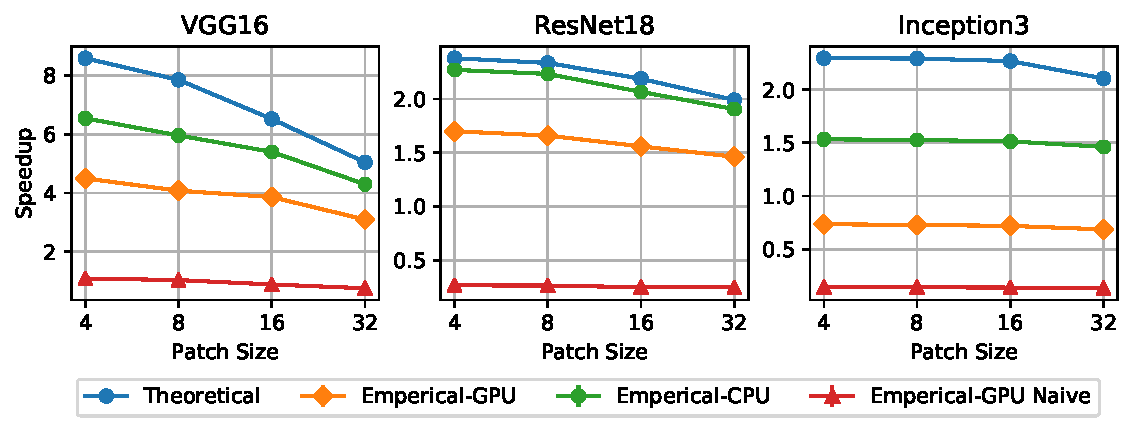
\includegraphics[width=\columnwidth]{images/5_2_1_edited}
\vspace{-8mm}
\caption{Speedups with only the incremental inference optimization (occlusion patch stride $S=4$).}
\label{fig:5_2_1_edited}
\end{figure}

\vspace{2mm}
\noindent \textbf{Only Incremental Inference.} 
We vary the patch size and set the stride to $4$. Figure~\ref{fig:5_2_1_edited} shows the results. As expected, the speedups go down as the patch size increases. Empirical-GPU Naive yields no speedups because it does not use our GPU-optimized kernel, while Empirical-GPU does. But Empirical-CPU is closer to theoretical speedup and almost matches it on ResNet18. Thus, there is still some room for improvement to improve the efficiency of incremental inference in both environments.


\begin{figure}[t]
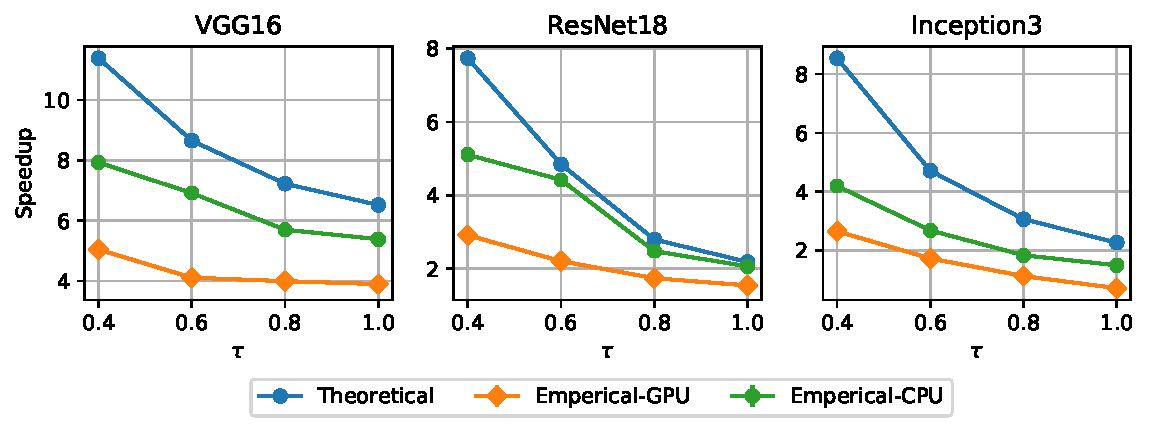
\includegraphics[width=\columnwidth]{images/5_2_2_edited}
\vspace{-8mm}
\caption{Speedups with incremental inference combined with only projective field thresholding (occlusion patch size$=16$, stride $S=4$).}
\label{fig:5_2_2_edited}
\end{figure}

\vspace{2mm}
\noindent \textbf{Projective Field Thresholding.} We vary $\tau$ from $1.0$ (no approximation) to $0.4$. Adaptive drill-down is disabled but note that this optimization builds on top of our incremental inference. The occlusion patch size is $16$ and stride is $4$. Figure~\ref{fig:5_2_2_edited} shows the results. The speedups go up steadily as $\tau$ drops for all 3 CNNs. Once again, Empirical-CPU nears the theoretical speedups on ResNet18, but the gap between Empirical-GPU and Empirical-CPU remains due to the disproportionate impact of memory stalls on GPU. Overall, this approximation offers some speedups in both environments, but has a higher impact on CPU than GPU.

\begin{figure}[t]
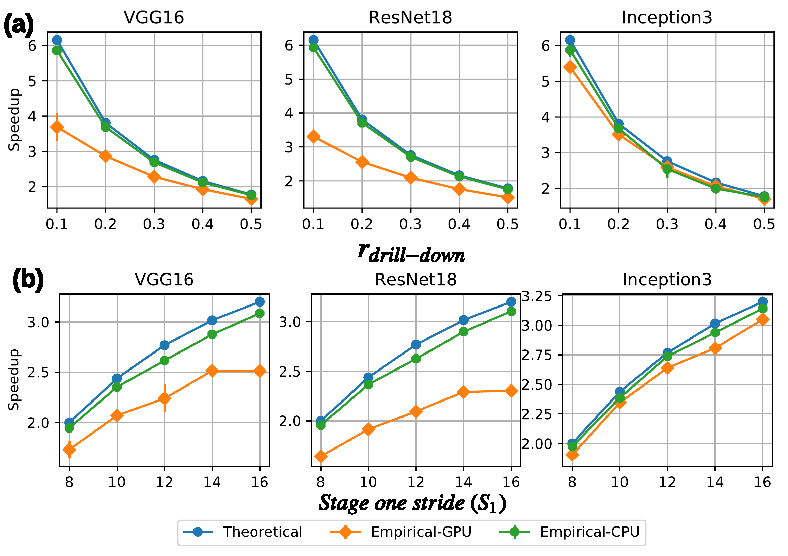
\includegraphics[width=\columnwidth]{images/5_2_3_edited}
\vspace{-8mm}
\caption{Speedups with incremental inference combined with adaptive drill-down. For (a), we set $S_1=16$. For (b), we set $r_{drill\_down}=0.25$).}
\label{fig:5_2_3_edited}
\end{figure}

\vspace{2mm}
\noindent \textbf{Adaptive Drill-Down.} Finally we study the effects of adaptive drill-down (again, on top of incremental inference) and disable projective field thresholding. The occlusion patch size is $16$. Stage two stride is $S_2 = 4$. First, we vary $r_{drill-down}$, while fixing stage one stride ($S_1 = 16$). Figure~\ref{fig:5_2_3_edited}(a) shows the results. Next, we vary $S_1$, while fixing $r_{drill-down} = 0.25$. Figure~\ref{fig:5_2_3_edited}(b) shows the results. As expected, the speedups go up as $r_{drill-down}$ goes down or $S_1$ goes up, since fewer re-inference queries arise in both cases. Empirical-CPU almost matches the theoretical speedups across the board; in fact, even Empirical-GPU almost matches theoretical speedups on Inception3. Empirical-GPU flattens out at high $S_1$, since the number of re-inference queries drops, thus resulting in diminishing returns for the benefits of batched execution on GPU. Overall, this optimization has a major impact on speeding up OBE for all CNNs in both environments.

\vspace{2mm}
\noindent \textbf{Summary of Experiments.} Overall, our empirical evaluation shows that \system~ is able to substantially accelerate the OBE workload for explaining CNN predictions, up to $16$X speedups on GPU and $34.5$X speedups on CPU. The speedups of all 3 of our optimizations depend on the CNN's architectural properties. The speedups of our approximate inference optimizations also depend on the dataset due to their tunable parameters, which \system ~can tune automatically. Finally, the speedups of \system ~are higher on CPU than GPU but the absolute runtimes are much lower on GPU. Overall, all of our optimizations in \system ~help reduce waiting times for users and can save resource costs, since they only using existing compute resources without forcing users to pay for more resources (say, renting more GPUs in the cloud).

\bibliographystyle{unsrt}
\bibliography{main}

%!TEX root = <main.tex>
\appendix

\section{Interactive Mode Execution}

\begin{figure}[t]
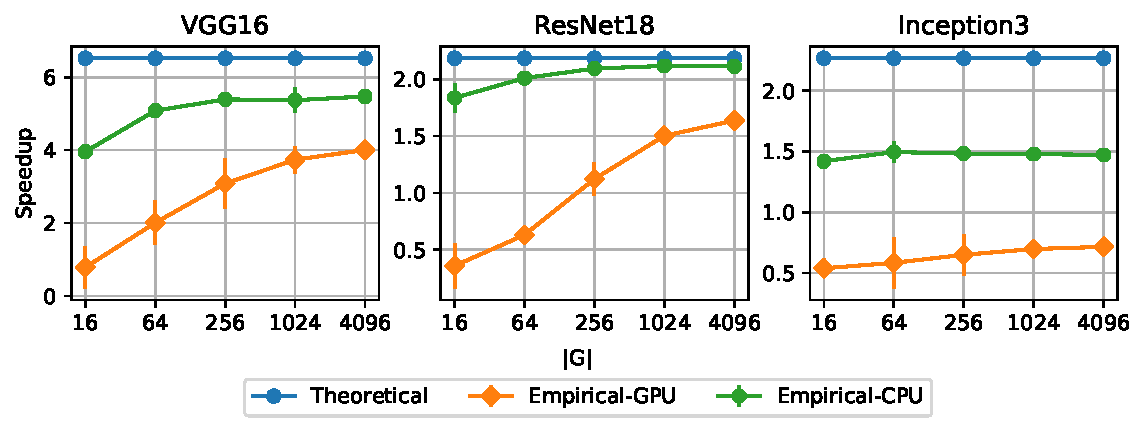
\includegraphics[width=\columnwidth]{images/interactive_experiment.pdf}
\vspace{-8mm}
\caption{Interactive mode execution of incremental inference with $G$s of different sizes}
\label{fig:interactive_experiment}
\end{figure}

We evaluate interactive-mode incremental inference execution (no approximate inference optimizations) with $G$s of different sizes.
Similar to non-interactive mode experiments presented in Section 5, all experiments are run in batched mode with a batch size of 16 for CPU based experiments and a batch size 128 for GPU based experiments.
If the size of $G$ (formally $|G|$) or the remainder of $G$ is smaller than the batch size, that value is used as the batch size (e.g. $|G| = 16$ results in a batch size of 16).
Figure \ref{fig:interactive_experiment} presents the final results.

\section{GPU-Optimized Kernel Implementation}

\begin{figure}[t]
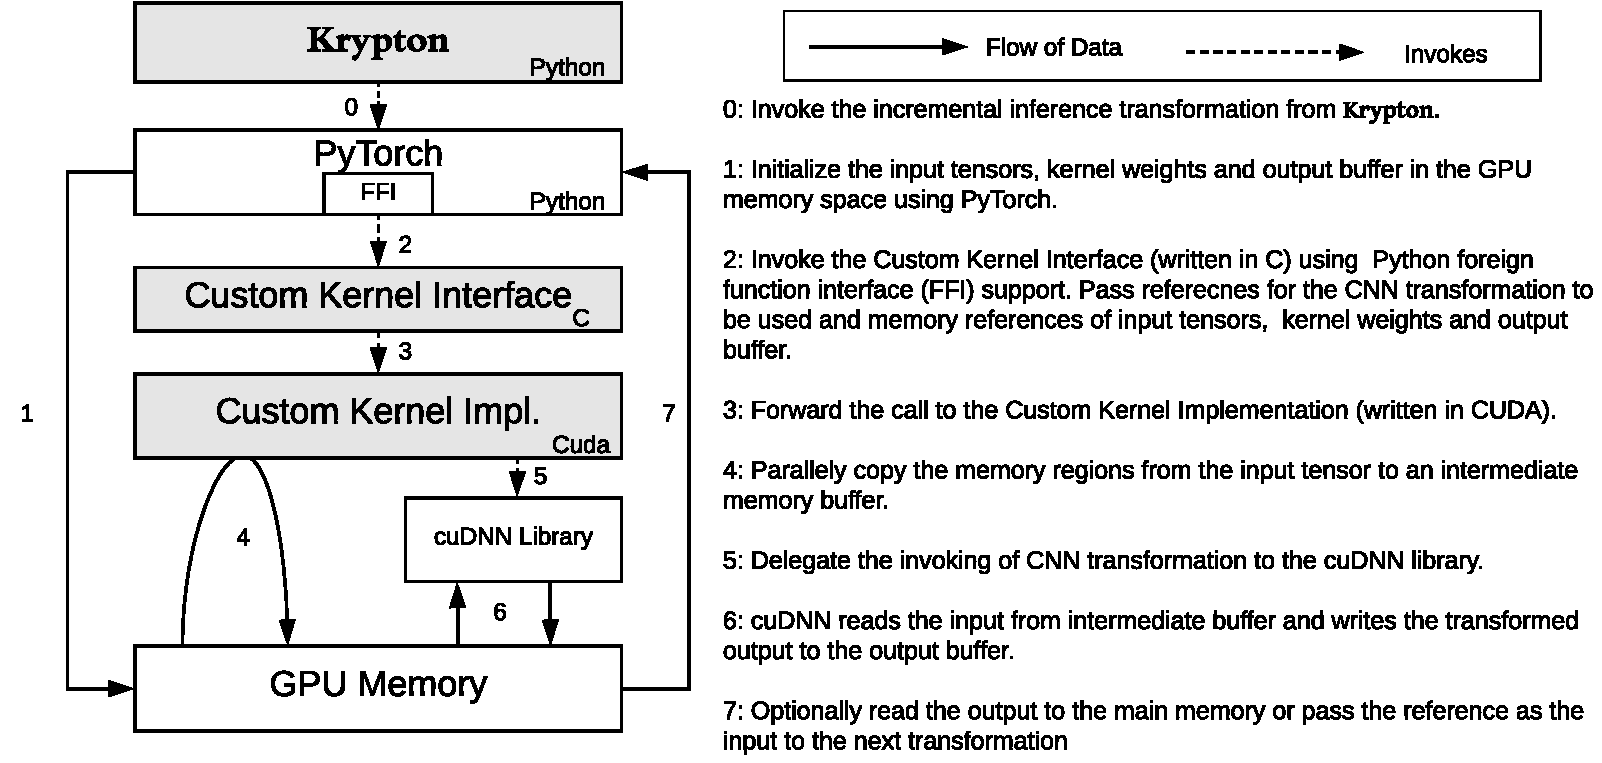
\includegraphics[width=\columnwidth]{images/gpu_kernel_impl.pdf}
\vspace{-8mm}
\caption{Custom GPU Kernel integration architecture}
\label{fig:custom_kernel_integration}
\end{figure}

We extend PyTorch by adding a custom GPU kernel which optimizes the input preparation for \textit{incremental inference} by invoking parallel memory copy operations.
This custom kernel is integrated to PyTorch using Python foreign function interface (FFI).
Python FFI integrates with the Custom Kernel Interface layer which intern invokes the Custom Kernel Implementation.
The high-level architecture of the Custom Kernel integration is shown in Figure~\ref{fig:custom_kernel_integration}


\section{Special Cases for Incremental Inference}

\begin{figure}[t]
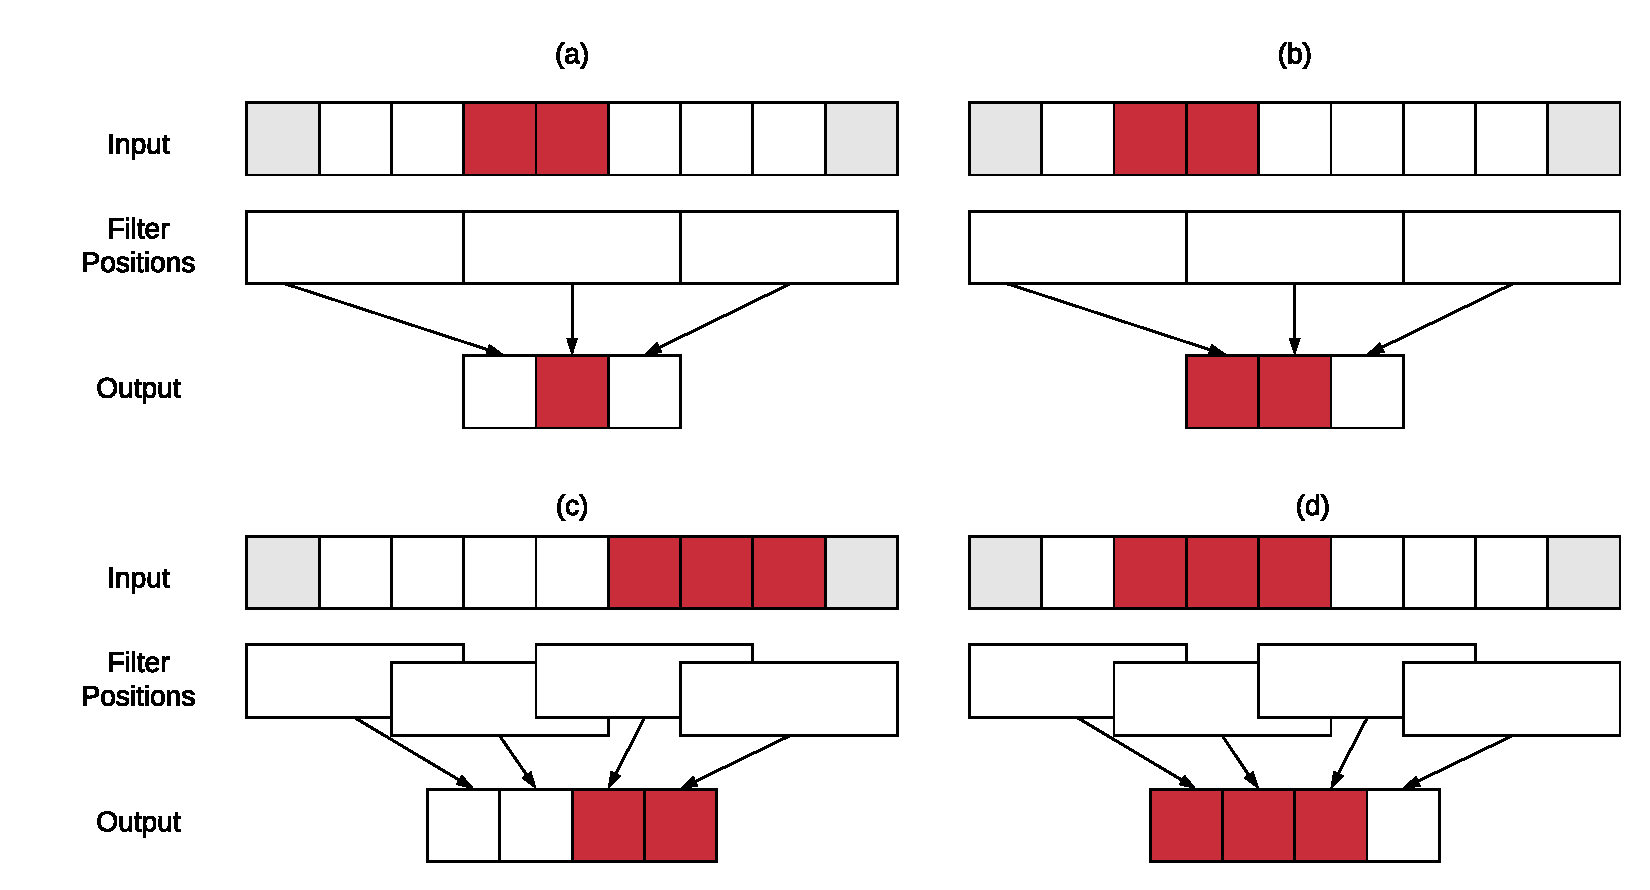
\includegraphics[width=\columnwidth]{images/less_one_example}
\vspace{-6mm}
\caption{1-D illustration of special cases for which actual output size will be smaller than the value given by Equation~(\ref{eqn:xcoordinate}). (a) and (b) show cases where the filter stride is equal to the filter size. (c) and (d) show situations where the position of the modified patch affecting the size of the output patch.}
\vspace{-4mm}
\label{fig:less_one_example}
\end{figure}

There are special cases under which the output patch size can be smaller than the values calculated in Section~\ref{sec:inc_computation}. Consider the simplified 1-D case shown in Figure~\ref{fig:less_one_example} (a), where the filter stride\footnote{Note that stride is typically less than or equal to filter size.} (3) is the same as the filter size (3). In this case, the size of the output update patch is one less than the value calculated by Equation~(\ref{eqn:patchwidth}). But this is not the case for the situation shown Figure~\ref{fig:less_one_example} (b), which has the same input patch size but placed at a different location.
% This issue arises only when the stride value is same as the filter size.
Another case arises when the modified patch is placed at the edge of the input, as shown in Figure~\ref{fig:less_one_example} (c). In this case, it is impossible for the filter to move freely through all positions, since it hits the input boundary. However, it is not the case for the modified patch shown in Figure \ref{fig:less_one_example} (d). In \system, we do not treat these cases separately but rather use the values calculated by Equation~(\ref{eqn:patchwidth}) for the width dimension (similarly for the height dimension), since they act as an upper bound. In the case of a smaller output patch, \system~ reads and updates a slightly bigger patch to preserve uniformity. This also requires updating the starting coordinates of the patch, as shown in Equation~(\ref{eqn:width_subtract}). This sort of uniform treatment is required for performing batched inference operations, which gives significant speedups compared to per-image inference.

\vspace{-4mm}
\begin{align}
\begin{split}
\label{eqn:width_subtract}
&\text{If~} x^\mathcal{O}_\mathcal{P} + ~W^\mathcal{O}_\mathcal{P} > W_{\mathcal{O}}:\\
&x^\mathcal{O}_\mathcal{P} ~ =  W_{\mathcal{O}} - W^\mathcal{O}_\mathcal{P}; 
x^\mathcal{I}_\mathcal{P} ~ = W_{\mathcal{I}} - W^\mathcal{I}_\mathcal{P}; 
x^\mathcal{R}_\mathcal{P} ~ = W_{\mathcal{I}} - W^\mathcal{R}_\mathcal{P}
\end{split}
\end{align}


\section{Effective Projective Field Size (1-D Scenario)}

We formalize the effective projective field growth for the one dimensional scenario with $n$ convolution layers (assuming certain conditions). This proof is motivated by a similar proof in \cite{luo2016understanding} which characterizes the effective growth rate of the receptive field in a CNN.

The input is $u(t)$ where
\begin{align}
	u(t) = 
	\begin{cases}
		1, & t = 0\\
		0, & t \neq 0 
	\end{cases}
\end{align}
and $t = 0, 1, -1, 2, -2, ...$ indexes the input pixels.

Each layer has the \textbf{same kernel} $v(t)$ of size $k$. The kernel signal can be formally defined as
\begin{align}
	v(t) = \sum_{m=0}^{k-1} w(m)\delta(t-m)
\end{align}
where $w(m)$ is the weight for the $m^{th}$ pixel in the kernel.
Without loosing generality, we can assume the weights are normalized, i.e. $\sum_{m}w(w)=1$. The output signal of the $n^{th}$ layer $o(t)$ is simply $o = u * v * ... * v$, convolving $u$ with $n$ such $v$s.
To compute the convolution, we can use the Discrete Time Fourier Transform to convert the signals into the Fourier domain, and obtain
\begin{align}
\begin{split}
	U(\omega) =&~ \sum_{t=-\infty}^{\infty} u(t)e^{-j\omega t} = 1, ~V(\omega) \\=&~ \sum_{t=-\infty}^{\infty} v(t)e^{-j\omega t} = \sum_{m=0}^{k-1} w(m)e^{-j\omega t}
\end{split}
\end{align}

Applying the convolution theorem, we have the Fourier transform of $o$ is
\begin{align}
\begin{split}
	\mathcal{F}(o) =&~ \mathcal{F}(u*v*...*v)(\omega) = U(\omega) . V(\omega)^n \\=&~ \Bigg(\sum_{m=0}^{k-1}w(m)e^{-j\omega t}\Bigg)^n
\end{split}
\end{align}

With inverse Fourier transform
\begin{align}
	o(t) = \frac{1}{2\pi}\int_{-\pi}^{\pi}\Big(\sum_{m=0}^{k-1}w(m)e^{-j\omega t}\Big)^ne^{j\omega t} d\omega
\end{align}

The space domain signal $o(t)$ is given by the coefficients of $e^{-j\omega t}$.
These coefficients turn out to be well studied in the combinatorics literature \cite{eger2013restricted}.
It can be shown that if $\mathbf{\sum_{m}w(m) = 1}$  and $\mathbf{w(m) \geq 0 ~\forall~ m}$ , then
\begin{align}
\begin{split}
	o(t) =&~ p(S_n=t)\\ 
	\text{where}~ S_n =&~ \sum_{i=1}^{n} X_i ~\text{and}~p(X_i=m) = w(m)
\end{split}
\end{align}

From the central limit theorem, as $n \rightarrow~\infty$, $\sqrt{n}(\frac{1}{n}S_n - \mathop{\mathbb{E}}[X]) \sim \mathcal{N}(0, Var[X])$ and $S_n \sim \mathcal{N}(n\mathop{\mathbb{E}}[X]), nVar[X])$.
As $o(t) = p(S_n=t)$, $o(t)$ also has a Gaussian shape with
\begin{align}
	\mathop{\mathbb{E}}[S_n] =&~ n\sum_{m=0}^{k-1}mw(m)\\
	Var[S_n] =&~ n \Bigg(\sum_{m=0}^{k-1}m^2w(m) - \Big(\sum_{m=0}^{k-1}mw(m)\Big)^2 \Bigg)
\end{align}

This indicates that $o(t)$ decays from the center of the projective field squared exponentially according to the Gaussian distribution.
As the rate of decay is related to the variance of the Gaussian and assuming the size of the effective projective field is one standard deviation, the size can be expressed as
\begin{align}
	\sqrt{Var[S_n]} = \sqrt{nVar[X_i]} = O(\sqrt{n})
\end{align}

On the other hand stacking more convolution layers would grow the theoretical projective field linearly. But the effective projective field size is shrinking at a rate of $O(1/\sqrt{n})$.


\section{Fine-tuning CNNs}

For \textit{OCT} and \textit{Chest X-Ray}, the 3 ImageNet-trained CNNs are fine-tuned by retraining the final Fully-Connected layer.
We use a train-validation-test split of 60-20-20 and the exact numbers for each dataset are shown in Table \ref{tbl:dataset_sizes}.
Cross-entropy loss with L2 regularization is used as the loss function and  Adam \cite{kingma2014adam} is used as the optimizer.
We tune learning rate $\eta \in [10^{-2}, 10^{-4}, 10^{-6}]$ and regularization parameter $\lambda \in [10^{-2}, 10^{-4}, 10^{-6}]$ using the validation set and train for 25 epochs.
Table \ref{tbl:finetune_accuracies} shows the final train and test accuracies.

\begin{table}[ht]
\begin{tabular}{cccc}
 & Train & Validation & Test \\ \hline
\hline
OCT & 50,382 & 16,853 & 16, 857 \\ \hline
Chest X-Ray & 3,463 & 1,237 & 1,156 \\ \hline
\end{tabular}
\caption{Train-validation-test split size for each dataset.}
\vspace{-6mm}
\label{tbl:dataset_sizes}
\end{table}

\begin{table}[ht]
\begin{tabular}{|c|l|l|l|l|l|l|}
\hline
\multicolumn{1}{|l|}{\multirow{3}{*}{}} & \multirow{3}{*}{Model} & \multicolumn{2}{l|}{\multirow{2}{*}{Accuracy(\%)}} & \multicolumn{3}{l|}{\multirow{2}{*}{Hyperparams.}} \\
\multicolumn{1}{|l|}{} &  & \multicolumn{2}{l|}{} & \multicolumn{3}{l|}{} \\ \cline{3-7} 
\multicolumn{1}{|l|}{} &  & Train & Test & \multicolumn{2}{l|}{$\eta$} & $\lambda$ \\ \hline
\multirow{3}{*}{OCT} & VGG16 & 79 & 82 & \multicolumn{2}{l|}{$10^{-4}$} & $10^{-4}$ \\ \cline{2-7} 
 & ResNet18 & 79 & 82 & \multicolumn{2}{l|}{$10^{-2}$} & $10^{-4}$ \\ \cline{2-7} 
 & Inception3 & 71 & 81 & \multicolumn{2}{l|}{$10^{-2}$} & $10^{-6}$ \\ \hline
\multirow{3}{*}{Chest X-Ray} & VGG16 & 75 & 76 & \multicolumn{2}{l|}{$10^{-4}$} & $10^{-4}$ \\ \cline{2-7} 
 & ResNet18 & 78 & 76 & \multicolumn{2}{l|}{$10^{-4}$} & $10^{-6}$ \\ \cline{2-7} 
 & Inception3 & 74 & 76 & \multicolumn{2}{l|}{$10^{-4}$} & $10^{-2}$ \\ \hline
\end{tabular}
\caption{Train and test accuracies after fine-tuning.}
\vspace{-6mm}
\label{tbl:finetune_accuracies}
\end{table}


\section{Deep CNN Explainability}
% With image recognition models, natural question is if the model is truly identifying objects in the image or just using surrounding or other objects for making false prediction.
Various approaches used to explain CNN predictions can be broadly divided into two categories, gradient-based and perturbation based approaches. Gradient-based approaches generate a sensitivity heat map by computing the partial derivatives of model output with respect to every input pixel via backpropagation.
In perturbation based approaches the output of the model is observed by modifying regions on the input image and thereby identify the sensitive regions.
% Even though gradient approaches require only a single forward inference and a single backpropagation to generate the sensitivity heat map, the output may not be very intuitive and hard to understand because the salient pixels tend to spread over a very large area of the input image.
Despite being time-consuming, in most real world use cases such as in medical imaging, practitioners tend to use occlusion experiments, a perturbation based approach, as the preferred approach for explanations as they produce high quality fine grained sensitivity heat maps using a process which is very intuitive to the human observer ~\cite{zeiler2014visualizing,jung2017deep,miller2017explanation}.


\section{Visual Examples}

Figure \ref{fig:visual_examples} presents occlusion heat maps for a sample image from each dataset with (a) \textit{incremental inference} for different \textit{projective field threshold} values and (b) \textit{incremental inference} with \textit{adaptive drill-down} for different \textit{projective field threshold} values. The predicted class label for \textit{OCT}, \textit{Chest X-Ray}, and \textit{ImageNet} are DME, VIRAL, and OBOE respectively.

\begin{figure*}[t]
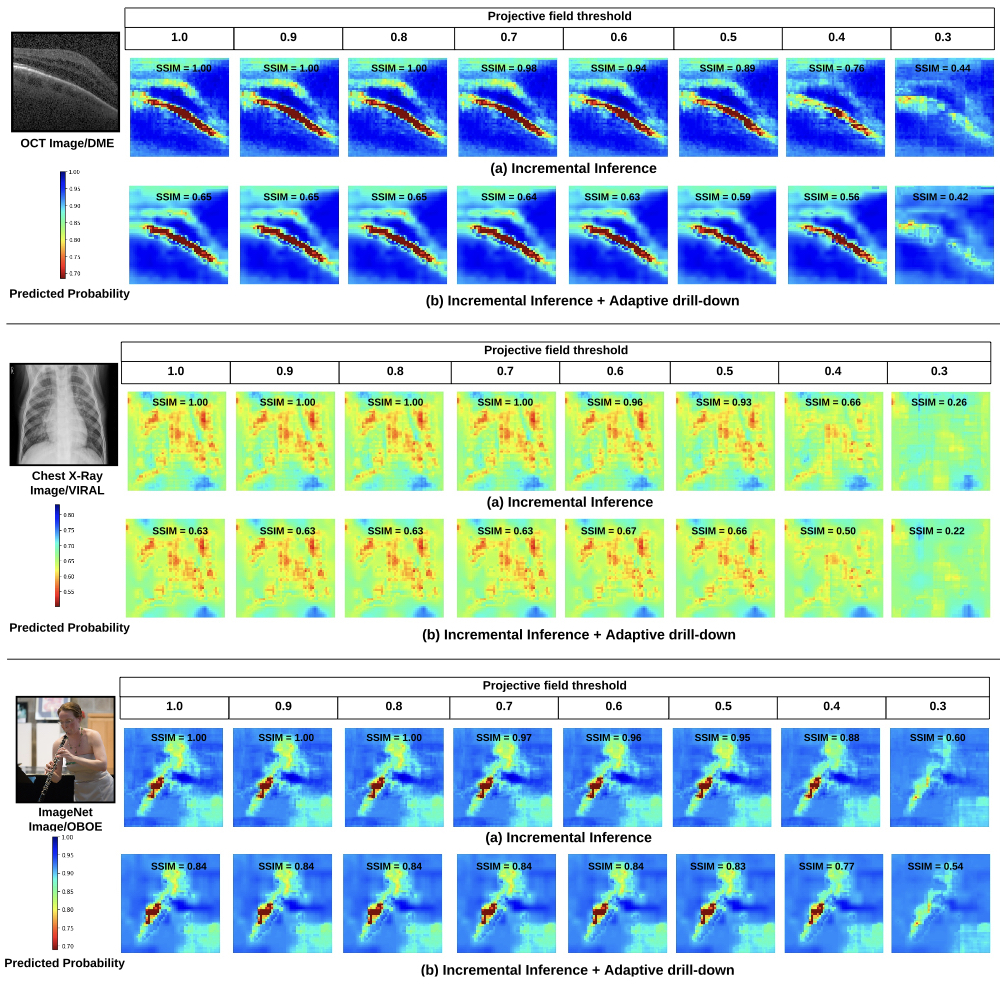
\includegraphics[width=\textwidth]{visualsjpeg}
%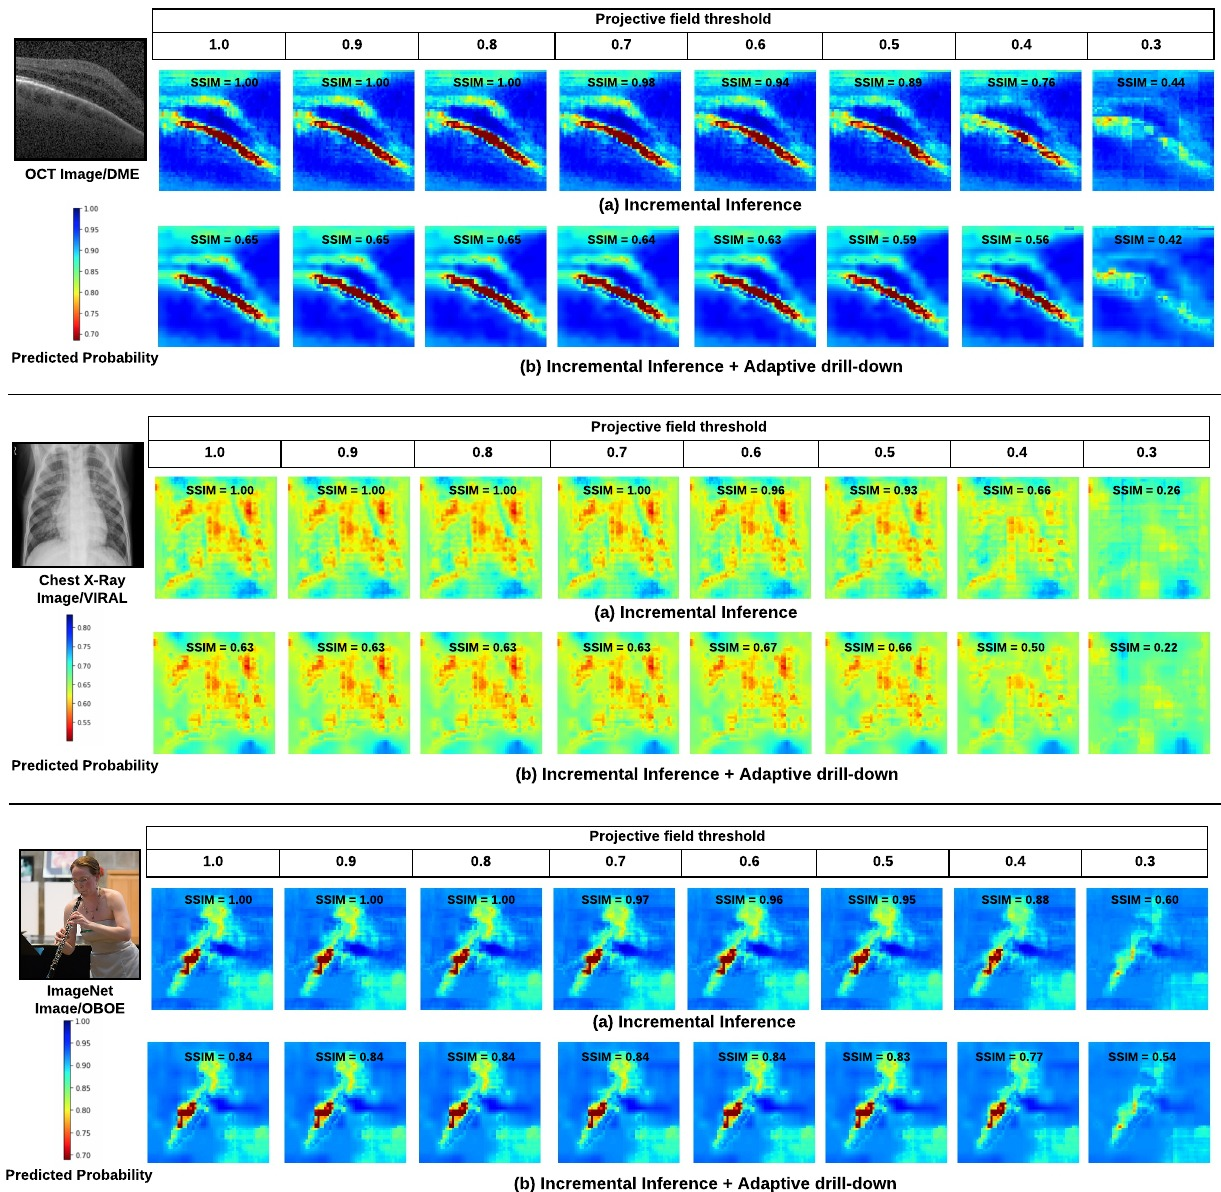
\includegraphics[width=\textwidth]{images/visual_examples}
\caption{Occlusion heat maps for sample images (CNN model = VGG16, occlusion patch size = 16, patch color = black, occlusion patch stride $(S~or~S_2)$ = 4. For \textit{OCT} $r_{drill\_down}=0.1$ and $\mathit{target}=5$. For \textit{Chest X-Ray} $r_{drill\_down}=0.4$ and $\mathit{target}=2$. For \textit{ImageNet} $r_{drill\_down}=0.25$ and $\mathit{target}=3$).}
\label{fig:visual_examples}
\end{figure*}
\end{document}